%!TEX program = xelatex
% !BIB program = bibtex
\documentclass[12pt,letterpaper]{article}
\usepackage{./style/dsc180reportstyle} % import dsc180reportstyle.sty

\newtheorem{theorem}{Theorem}[section]
\newtheorem{corollary}{Corollary}[theorem]
\newtheorem{definition}{Definition}

%%%%%%%%%%%%%%%%%%%%%%%%%%%%%%%%%%%%%%%%%%%%%%%%%%%%%%%%
%%%% Title and Authors
%%%%%%%%%%%%%%%%%%%%%%%%%%%%%%%%%%%%%%%%%%%%%%%%%%%%%%%%

\title{Privacy in Practice: The Feasibility of Differential Privacy for Telemetry Analysis}

\author{Trey Scheid \\
  {\tt tscheid@ucsd.edu} \\\And
  Tyler Kurpanek \\
  {\tt tkurpane@ucsd.edu} \\\And
  Bradley Nathanson \\
  {\tt bnathanson@ucsd.edu} \\\And
  Christopher Lum \\
  {\tt cslum@ucsd.edu} \\\And
  Yu-Xiang Wang \\
  {\tt yuxiangw@ucsd.edu} \\}

\begin{document}
% INSERT TITLE
% title is defined above
\maketitle



%%%%%%%%%%%%%%%%%%%%%%%%%%%%%%%%%%%%%%%%%%%%%%%%%%%%%%%%
%%%% Abstract and Links
%%%%%%%%%%%%%%%%%%%%%%%%%%%%%%%%%%%%%%%%%%%%%%%%%%%%%%%%

\begin{abstract}    
  This research investigates the implementation implications of differential privacy mechanisms for telemetry data analysis, with a focus on real-world applications. We show, through examples, how knowledge of fundamental privacy-preserving techniques, including randomized response and the Laplace mechanism, is enough to protect sensitive information while maintaining analytical utility. We privatize data tasks from 4 applied research works using Intel telemetry data which   encompasses multiple statistical tasks, from user-level rate analysis to logistic regression classification. The study utilizes various $(\epsilon, \delta)$ budgets (using AutoDP) for precise privacy loss measurement and to quantify the inherent tradeoff between privacy and utility. By demonstrating the feasibility of differential privacy in production environments, we provide a roadmap for organizations seeking to enhance their privacy practices.
  \begin{center}
    Website: \url{https://trey-scheid.github.io/privacy-in-practice/} \\
    Code: \url{https://github.com/Trey-Scheid/privacy-in-practice}
  \end{center}
\end{abstract}

\clearpage

% TABLE OF CONTENTS
{\Large\bf\raggedright Table of Contents}

\maketoc

\clearpage

%%%%%%%%%%%%%%%%%%%
%%%% INTRO %%%%%%%%%%%
%%%%%%%%%%%%%%%%%%%

\section{Introduction}

The implementation of differential privacy in production environments presents significant challenges in balancing privacy guarantees with analytical utility. This research addresses these challenges by developing practical privacy-preserving mechanisms for existing telemetry analysis tasks while maintaining the usefulness of their systems. We integrate various differential privacy mechanisms including: Gaussian Composition, the Exponential\/Laplace mechanism, and DP-GD to protect sensitive information in telemetry data. Our chosen data tasks encompasses multiple statistical tasks, from user-level rate analysis to logistic regression classification correlation. By evaluating the trade-offs between privacy guarantees and analytical accuracy in production settings, we provide evidence and direction for organizations looking to enhance their privacy practices.

\subsection{Motivation}

Despite the growing importance of privacy-preserving data analysis \cite{PewPrivacy2019}, many practitioners perceive differential privacy implementation as complex and challenging, others note how results only come with dissatisfactory $\epsilon$-level guarantees \cite{FLandPrivacy}. Besides the sub-optimality of some DP methods, this perception stems from human difficulties: the mathematical complexity of privacy definitions, the need to carefully calibrate privacy parameters, and concerns about reduced utility (managing the trade-off) \cite{DP-fyML}. Researchers are working to democratize, demystify, and improve usability around Differential Privacy \cite{DP-fyML}. Recent developments have significantly lowered these barriers to entry. Tools like Google's Privacy on Beam \footnote{\url{https://codelabs.developers.google.com/codelabs/privacy-on-beam}}, Microsoft's SmartNoise \footnote{\url{https://smartnoise.org}}, and various open-source libraries like AutoDP\footnote{\url{https://pypi.org/project/autodp/}} provide accessible frameworks for implementing differential privacy. These tools abstract away much of the underlying complexity while maintaining rigorous privacy guarantees. In addition, educational resources and practical tutorials have emerged to guide practitioners through implementation challenges \footnote{\url{https://desfontain.es/blog/friendly-intro-to-differential-privacy.html}}.

%"has been observed that limiting sensitivity even with small amounts of noise (or no noise at all) can significantly reduce memorization.18 This gap is to be expected, as DP assumes a “worst-case adversary’’ with infinite computation and access to arbitrary side information. These assumptions are often unrealistic in practice. Thus, there are substantial advantages to training using a DP algorithm that limits each user’s influence, even if the explicit random noise introduced into the training process is not enough to ensure a small ε formally. Nevertheless, designing practical FL and FA algorithms that achieve small ε guarantees is an important area of ongoing research."

This research builds upon these recent developments by providing a practical demonstration of differential privacy mechanisms in telemetry data analysis. By implementing privacy-preserving techniques for existing tasks, we aim to show that differential privacy can be seamlessly integrated into production systems without significant utility loss. Our work focuses on two key objectives: privatizing existing telemetry analysis tasks and evaluating the privacy-utility tradeoffs in production settings.

\subsection{Differential Privacy}

Differential privacy by \cite{DworkRoth} is a framework for data privacy that gives a mathematical guarantee that the information for each individual (record or user) in the dataset is protected\footnote{\cite{DP-def} has an in depth explanation of interpretations and attacks.}. The core idea is to introduce random noise into algorithms so that the data of any individual does not significantly affect the overall result and therefore is not recoverable or identifiable. 

Mathematically, a mechanism $M$ is considered $(\epsilon, \delta)$ differentially private if for all datasets $D$ and $D'$ which differ by at most 1 element when $\P [ M(D)\in S ] \leq e^\epsilon \P [ M(D') \in S)] + \delta$ where $\epsilon$ and $\delta$ are privacy parameters and $S$ is a query solution set. Smaller $\epsilon$ and $\delta$ imply stronger privacy guarantees. Differential privacy is a \textit{property} of algorithms, not datasets; it is a method that ensures private results to a high degree of probability (whether that is a trained model or a noisy dataset). 

This definition applies to data anonymization, but does not cover methods for transparency, use, access or security. By pursuing this property for common data tasks we aim to create a solution which once implemented achieves similar results but removes the need for data access and security. Some settings the predictions themselves are important, but sensitive, meaning a mechanism without anonymity is unusable!

\subsection{Telemetry Data}

The Intel Data Collection and Analysis (DCA) team derives insights from over 39 million systems! This includes any of their hardware installed in personal, corporate and IoT devices (collected only with consent). Through their partnership with the University of California San Diego's Halicioğlu Data Science Institute, at the foundation of Intel Lab's Telemetry Center of Excellence, they permit study of possibly sensitive device information to develop solutions that benefit the whole ecosystem \footnote{\url{https://community.intel.com/t5/Blogs/Tech-Innovation/Data-Center/Intel-Labs-Investment-in-Telemetry-Center-of-Excellence-Produces/post/1460669}}. Faculty and Intel researchers have published many white papers using the database since the CoE inception in 2020. We selected 4 of interest and found their core data science methods Table \ref{tab:DataTasks}.
It is important to note that all DCA data was collected without any personally identifiable information and assigned a random device identifier (GUID) to match records across the database. There is a strict EULA limiting the use of the DCA data to improving performance, and design of products. The studies replicated here all used a small sample of 10,000 unique GUIDs for their analysis, Intel verified results on the entire dataset for some afterwards.

\begin{table}[h]%!
\begin{center}
\caption{Data Tasks}
\label{tab:DataTasks}
\begin{tabular}{|p{4.5cm}|p{2.5cm}|p{5cm}|p{2.7cm}|}
    \hline
    Data Task & Code & Paper & Citation \\
    \hline
    Conditional Probabilities & COND\_PROB & Exploration of CPU Error Dependencies and Prediction & \cite{Kwasnick2023} \\
    \hline
    KMeans Clustering & KMEANS & PC Health Impact White Paper & \cite{kmeans} \\
    \hline
    Lasso Regression & LASSO & Power Consumption Patterns in Intel’s Telemetry Data: China Burns 2x Energy that of the US & \cite{lassocarbon} \\
    \hline
    Logistic Regression Significance Tests & LR\_PVAL & Product Health Insights Using Telemetry & \cite{prodhealLR} \\
    \hline
\end{tabular}
\end{center}
\end{table}

Differential privacy methods and guarantees are attractive for many domains. Telemetry is the remote data transfer of automated system measurements. As people use technology everyday their machines track usage diagnostics which are used by hardware and software manufacturers to reduce bugs and increase efficiency. System usage information is recorded at regular intervals and usually results in massive quantities of measurements. The identifiability of the specific machine or user of an event is a concern regardless of PIID tags. Dinur Nissim Reconstruction and linkage attacks can be used to recover or reconstruct the original information: the source \cite{DinurReconstruction}. This is a breach of privacy for a user which depending on the sensitivity of the information can be concerning. For example, personal laptops may send diagnostics to Intel given that the user opts in to the program [Intel telemetry]. 

We use a secure research database shared be Intel Corporation with consent of its users to generate real results.

\subsubsection{Errors}

In our paper, we will analyze two different types of errors. The Machine Check Architecture, or MCA, will detect an error and label it as either corrected or uncorrected. A corrected error means the system can observe and correct a detected error. Correction mechanisms include single error correction, double error correction, and more. An uncorrected error is one that was detected but not corrected or there was a computation delay long enough that the MCA treated it as an interrupted computation. \cite{Kwasnick2023}

\subsubsection{Hardware Power}

Another concept is device power usage, this is the rate of energy consumption by the hardware. The lasso task focuses analysis on U-series CPUs. Around 50 Watts of power is normal for these CPUs (this is comparable to an outdated or inefficient light bulb). One Watt is defined as 1 Joule / second: lower energy per time is better for battery life and thermal regulation, this leads to cleaner environmental impact. 

\subsection{Applications}

Telemetry is one narrow domain which privacy is a concern, many other types of data require sensitive handling and sharing practices. For example the US Census \footnote{\url{https://www.census.gov/about/policies/privacy/privacy-policy.html}}. 

We will get into the specifics of each task, however note that each one can be applied to datasets in any domain. Probabilities of political party affiliation, Lasso/kmeans for gene identification, or correlation for stock prices. 

\subsection{Related Work}

We are building on a previous analysis on differentially private mechanisms for Logistic Regression \cite{qtr1proj}. The paper investigates how privacy affects different mini-batch stochastic gradient descent algorithms for logistic regression classification. It is shown that privacy affects the batch size for optimal performance. The each task has unique methods that build on previous work as well. 

%%%%%%%%%%%%%%%%%%%
%%%%  METHODS  %%%%%%%%
%%%%%%%%%%%%%%%%%%%

\section{Methods}

\subsection{Utility}

Each method used in our study has different measures of success, but they can all be translated into a proportion representing utility compared to the best model, whether that is the non-private baseline or an improved version. In the context of differential privacy, utility refers to the degree to which a privatized model or analysis retains its analytical accuracy and usefulness compared to its non-private counterpart.


\subsection{Data Structure}

After identifying research tasks which are commonplace in analytics, we needed to start by replicating the tasks on the data. First the data needs ingestion and processing. One key feature of telemetry data is the volume; the Intel database consists of many tables that are already a processed version of raw device signals, aggregation and merges reduce the size. The database schema contains 10's of tables and diagnostic metrics, most require hardware and network domain knowledge. Intel Database documentation and the methods section of each paper were essential to replicate the works.

The tables once loaded to disc could be processed with SQL queries and filtered and processed with more basic operations such as aggregating by group and finding statistics. Each paper had its own processing steps and relevant tables which are stored as compressed files and then loaded into python for each task.

\subsection{LR\_PVAL: Private Correlation (via Logistic Regression Coefficient)}

This paper \cite{prodhealLR} seeks to identify whether a certain variable is disproportionately present for a certain outcome. 
More specifically, it takes a close look at two variables, max temperature on a day and whether a corrected error was present on that day. 
They would take one of those two variables and train a logistic regression model with maximum likelihood estimation to predict whether an uncorrected error was present.
From the model, they use the coefficient of the variable and make a hypothesis test whether that variable is equal to zero.

For our implementation, we focused only on whether there were corrected errors on a day, and not the variable max temperature on a day.
We add privacy to the model by using DP-SGD when training the logistic regression model, where the hypothesis test is then private by means of post-processing.
We replicated the non-private model to get a baseline for utility and compared it to our private model using set intersection over union.
Our data came from Intel's telemetry database, which contains information about the hardware and software on millions of devices
and we took a subset of one year of the data from Februrary 2020 to 2021.

\subsubsection{Nonprivate Logistic Regression}

The paper used a univariate logistic regression model, one for each of the top 30 uncorrected error codes.
The target variable is whether or not an uncorrected error was present on a day, 
and the feature a boolean of whether there was a corrected error on that day, 
making uncorrected error ~ corrected error.

The logistic regression model is defined as 

\begin{equation}
    \label{eq:logistic_regression}
    \log \frac{P(y=1|x)}{1-P(y=1|x)} = \beta_0 + \beta_1 x
\end{equation}

and they took $\beta_1$ as the coefficient of interest.
They used a Wald test to test the null hypothesis that $\beta_1 = 0$ against the alternative that $\beta_1 \neq 0$.
The Wald test statistic is defined as 

\begin{equation}
    \label{eq:wald_test}
    W = \frac{\hat{\beta}_1}{SE(\hat{\beta}_1)}
\end{equation}

where $\hat{\beta}_1$ is the coefficient estimate and $SE(\hat{\beta}_1)$ is the standard error of the coefficient estimate.
This statistic can be used to test whether or not the feature is significant in predicting the target variable (whether the presence of a corrected error is associated with the presence of an uncorrected error).
For our implementation, we used the statsmodels library to fit the model and calculate the coefficient and standard error with an alpha of 0.05.

\subsubsection{Private Logistic Regression}

In order to add privacy to the model, we used DP-Gradient Descent to train the model.
DP-GD is a method of training a model with differential privacy by adding noise to the gradient updates using Gaussian noise.
Each iteration of gradient descent adds a little bit more noise, consuming a proportion of the privacy budget, 
meaning that higher epsilons require more iterations.
We considered using DP-Stochastic Gradient Descent, but the processed datasets were small enough to warrant using DP-GD.
We implemented our own DP-GD algorithm using AutoDP\footnote{\url{https://pypi.org/project/autodp/}} to account for our privacy budget.
After privately training the model, post-processing enabled us to calculate the wald test the same way as in the non-private model.
In order to compare the alpha values, we completed permutation testing on each model in order to calculate the empirical p-value which was used to identify models that were statistically significant.
One of the thirty models had exceptionally more values than the others, so to save compute we removed it from the analysis.

\subsubsection{Utility}

We defined our utility metric as the set intersection over union of the top 29 uncorrected error codes.
This metric has a range of 0 to 1, where 0 is no intersection and 1 is full intersection,
meaning that the higher the utility, the more similar the two results are.


\subsection{KMEANS: Private Clustering (DP-Lloyd's)}

K-Means clustering (Lloyd's Algorithm) is applied to group devices based on similarities in their usage patterns. The method leverages Z-scores for standardizing the usage data and calculates L1 distances between weekly usage patterns to identify trends over time. Lloyd's Algorithm clusters devices by assigning them to centroids based on their usage patterns, recalculating the centroids as the mean of assigned points after each iteration. 

Differentially Private Lloyd's Algorithm (DP-Lloyd's)\footnote{\url{https://arxiv.org/pdf/1504.05998}} modifies the standard K-Means clustering by adding Laplacian noise during the iterative centroid update step to ensure privacy. It introduces noise to both the sum of coordinates and the count of points within clusters, with the amount of noise controlled by the number of iterations and the sensitivity of the data. This is applied after clipping the data, to for ensure that the impact of any single data point is limited. 
\[
\text{x'}_j = \text{clip}\left( \text{x}_j, -\tau, \tau \right)
\]

After clipping the data, the sum of each cluster is computed with added Laplace noise. \\
One point changes the sum, at most, the range of the dataset, which is \(2 \times \tau\) (the sensitivity). The number of data points is at least 1 if the cluster exists, and so one data point changes the count by 1. The sensitivity is therefore 1. These sensitivities are then divided by the per-iteration  $\epsilon$.

\[
\text{new\_centroid}_j=
\frac{
    \sum_{i=1}^{n_j} \text{x'}_{j,i} + \text{Lap}(\tau \times 2, \epsilon_{\text{iter}})
}{
    \max\left( 1, n_j + \text{Lap}(1, \epsilon_{\text{iter}}) \right)
}
\]

\subsubsection{Utility}
To calculate the utility for the K-Means task, we defined the loss for each
epsilon as the sum of squared distances between each data point and its closest centroid. We then divided it by the number of data point so it is agnostic to the dataset size. We then normalized the loss so that each loss value fell between 0 and 1 and defined the utility as
1-loss to inverse it.



\subsection{COND\_PROB: Private Conditional Probabilities (Laplace Mech)}

In order to replicate the paper, were are going to apply differential privacy methods to the processes outlined in the paper. In the paper, the authors first separate each GUID (user) into the number of corrected errors observed during a set time period. They then created a histogram where the x-axis was the number of corrected errors observed and the y-axis was the percentage of GUID's that observed an uncorrected error.\cite{Kwasnick2023} This is the process that we are aiming to privatize. 

We are releasing a percentage for each bin in the histogram, and in order to guarantee privacy, we must add noise to to both the numerator and denominator where the numerator is the number of GUID's that contained an uncorrected error (number of 1's) and the denominator is the number of GUID's total. However we can not release the number of GUID's in each corrected error count as that would violate differential privacy so instead we are just going to add noise to number of GUID's that contained an uncorrected error as well as the number of GUID's that did not contain an uncorrected an error (number of 1's + number of 0's) so that we have a private denominator. 

\[
P(Uncorrected) = \frac{\text{GUID's containing an Uncorrected Error}}{\text{Total GUID's}}
\]

We are going to apply the Laplace mechanism to to release this percentage privately. The Laplace mechanism adds noise drawn from the Laplace distribution to the output of a function. B is the scale parameter and $\nabla f$ is the sensitivity of the function f. \cite{DworkRoth}


$$noise \sim Lap(b) $$
$$Lap(x|b) = \frac{1}{2b}e^{-\frac{|x|}{b}}$$
$$b = \frac{\Delta f}{\epsilon}$$

The sensitivity of the function is defined as the maximum possible absolute change in the output of the function due to the change in a single user's data. Since we are dealing with a percentage (and we are considering the worst case), this change can be at most 1 user, which corresponds to a sensitivity of 1 (in terms of the scale of the count, not the percentage itself). This is because, in the worst case, the change is a single user being added or removed, and the total number of GUIDs is assumed to be large enough that the effect of one user's change on the output is not too significant.and $\nabla f$ is the privacy parameter. 
\begin{center}
$$\Delta f = \max_{D, D'} ||f(x) - f(x')|| = 1$$ \\
\text{D and D' are neighboring datasets}
\end{center}

\subsubsection{Utility}

To calculate the utility for the Conditional Probability task, we defined the loss for each epsilon as the Mean Absolute error between the Noisy and Original Histograms. We then normalized the loss so that each loss value fell between 0 and 1 and defined the utility as 1/loss. 

\subsection{LASSO Private $\ell$1 Regularized Regression (via DP-Frank-Wolfe)}

\subsubsection{Non-private Lasso Regression}

Lasso Regression (Least Absolute Shrinkage and Selection Operator) is a variant of linear regression which penalizes the size of the solution by its $\ell$1-norm. This means the model balances fitting the data with the size of the weights. It is known that depending on the level of regulation this results in a sparse solution, meaning many features are given no weight. This can be advantageous in many settings, it is used in an Intel Telemetry paper by \cite{lassocarbon} to identify key features that contribute to the response variable: cpu average power (Watts). 

The model is typically trained by solving the linear optimization problem Eq \ref{eq:estimator} with a penalty term added, iterative methods can approximate the solution very quickly.

Lasso regression minimizes the residual sum of squares Eq \ref{eq:Risk} subject to a constraint on the sum of the absolute values of the coefficients ($\ell$1 penalty). This penalty can shrink some coefficients exactly to zero, effectively removing irrelevant features from the model, making it particularly useful for high-dimensional data where feature selection is desired. The $\ell$1 regularization in Lasso encourages sparse models, unlike $\ell$2 regularization (Ridge regression) which merely shrinks coefficients without eliminating them.

Given a dataset $D = \{(x_1, y_1), \ldots, (x_n, y_n)\}$ of $n$ samples where $x_i \in \mathbb{R}^p$, $y_i \in \mathbb{R}$, and loss function:
\begin{equation}
    \label{eq:Loss}
    \mathcal{L}(\theta; D) = \frac{1}{n}\sum_{i=1}^{n}(x_i \cdot \theta - y_i)^2
\end{equation}

the LASSO estimator solves:
\begin{equation}
    \label{eq:estimator}
    \theta^* = {\arg \min}_{\theta: \space \|\theta\|_1 \leq \ell} \mathcal{L}(\theta; D)
\end{equation}

Minimizing the excess empirical risk:
\begin{equation}
    \label{eq:Risk}
    R(\theta; D) \stackrel{\text{def}}{=} \frac{1}{n}\sum_{i=1}^{n}\mathcal{L}(\theta; d_i) - \min_{\theta \in \mathcal{C}}\frac{1}{n}\sum_{i=1}^{n}\mathcal{L}(\theta; d_i)
\end{equation}


\subsubsection{Private Lasso Regression}

To solve the Lasso optimization problem while ensuring differential privacy, we implemented the Frank-Wolfe algorithm Alg \ref{alg:DP-FW} as described in the Nearly-Optimal Private Lasso paper \cite{NIPS2015_52d080a3}. The standard (not privatized) Frank-Wolfe algorithm Alg \ref{alg:FW} is an iterative, first-order optimization method for constrained convex optimization. In each iteration, it considers a linear approximation of the objective function and traverses along this over the same domain. Unlike gradient descent methods that require projection steps, Frank-Wolfe naturally stays within the feasible set, making it particularly suitable for problems with $\ell$1 constraints like Eq \ref{eq:Loss}. The algorithm iteratively computes the gradient of the loss function at the current point, finds the vertex of the constraint set that minimizes the inner product with this gradient, and then takes a convex combination of the current point and this vertex.

% Algorithm 1: Frank-Wolfe algorithm
\begin{algorithm}[H]
    \DontPrintSemicolon
    \caption{Frank-Wolfe algorithm}
    \label{alg:FW}
    % \KwIn{$\mathcal{C} \subseteq \mathbb{R}^{p}$, $\mathcal{L}: \mathcal{C} \rightarrow \mathbb{R}$, $\mu_{t}$}
    Choose an arbitrary $\theta_{1}$ from $\mathcal{C}$\;
    \For{$t=1$ \KwTo $T-1$}{
        Compute $\widetilde{\theta}_{t}=\operatorname{argmin}_{\theta \in \mathcal{C}}\left\langle\nabla \mathcal{L}\left(\theta_{t}\right),\left(\theta-\theta_{t}\right)\right\rangle$\;
        Set $\theta_{t+1}=\theta_{t}+\mu_{t}\left(\widetilde{\theta}_{t}-\theta_{t}\right)$\;
    }
    \KwRet{$\theta_{T}$}\;
\end{algorithm}

To privatize the Frank-Wolfe algorithm, we incorporated the exponential mechanism. The exponential mechanism Def \ref{def:ExpMech} (\cite{ExpMech}) selects an output with probability proportional to the exponential of a utility function, which measures the quality of each possible output. In our implementation, at each iteration of Frank-Wolfe, instead of deterministically selecting the vertex that minimizes the inner product with the gradient, we use the exponential mechanism to probabilistically select a vertex, adding noise proportional to the sensitivity of the selection process Thm \ref{thm:dp}. The exponential mechanism tends to select outputs with higher utility scores with higher probability. The resulting algorithm achieves an excess risk of approximately $O(1/n^{(2/3)})$, proven to be nearly optimal for private Lasso regression Thm \ref{thm:NearOpt}.

% 2
\begin{algorithm}[H]
    \DontPrintSemicolon
    \caption{Differentially Private Frank-Wolfe Algorithm via Exponential Mechanism}
    \label{alg:DP-FW}
    %Data set: $\mathcal{D}=\left\{d_{1}, \cdots, d_{n}\right\}$, loss function: $\mathcal{L}(\theta; D)=\frac{1}{n} \sum_{i=1}^{n} \mathcal{L}\left(\theta; d_{i}\right)$ 
    \KwIn{$L_{1}$: $\ell_{1}$-Lipschitz constant  for $\mathcal{L}$, convex set: $\mathcal{C}=\operatorname{conv}(S)$ with $\|S\|_{1}$ denoting $\max_{s \in S}\|s\|_{1}$}
    
    Choose an arbitrary $\theta_{1}$ from $\mathcal{C}$\;
    
    \For{$t=1$ \KwTo $T-1$}{
        Compute gradient $g_t = \nabla \mathcal{L}(\theta_t; D)$\;
        
        \tcc{Exponential Mechanism to select vertex}
        \For{each vertex $s \in S$}{
            Compute quality score $q_s = -\langle s, g_t \rangle$\;
            \tcc{Higher quality = lower inner product with gradient}
        }
        
        Set sensitivity $\Delta = \frac{L_1\|S\|_1}{n}$\;
        
        Sample $\widetilde{\theta}_t$ from $S$ with probability proportional to:\;
        $\Pr[\widetilde{\theta}_t = s] \propto \exp\left(\frac{\epsilon q_s}{2\Delta\sqrt{8T\log(1/\delta)}}\right)$\;
        
        $\theta_{t+1} \leftarrow (1-\mu_t)\theta_t + \mu_t\widetilde{\theta}_t$, where $\mu_t = \frac{2}{t+2}$\;
    }
    
    \KwRet{$\theta^{\text{priv}} = \theta_T$}\;
\end{algorithm}

\cite{NIPS2015_52d080a3} Private Frank-Wolfe Lasso Alg \ref{alg:DP-FW} limits excess risk (worse performance compared to non-private baseline) according to Thm \ref{thm:utilcor} for lasso regression with bounded features ($\|x\|_{\infty} \leq 1$ and $|y| \leq 1$). (See \cite{lassocarbon} for proofs)


\subsubsection{Telemetry Application}

\citeauthor{lassocarbon} analyzed the telemetry data to help Intel lower their carbon emissions. To target their development on areas of highest impact, lasso is used to identify features that best predict high power usage. Features include user behavior variables, such as software categories, web usage categories, and user personas. Features also has device properties like number of cores, device age, screen size, model vendor and manufacturer. Each device is given an internal identification number (GUID). Features for this task are normalized and aggregated to be one stat per device per day. See their work for more details. 

Response Variable is a weighted average of signals:

\[power\_mean = \frac{\text{SUM}(\text{nrs} \cdot \text{mean})}{\text{SUM}(\text{nrs})}\]

From the database nrs is the number of samples and mean is the power signal. 

\subsubsection{Utility}

To analyze private performance across many tasks, we transform the prediction error into a normalized utility metric. Lasso regression naturally reports mean square error on a test set of data. Error therefore falls in the domain $(0, \infty)$, so we set a reasonable maximum error we expect would be considered a model with 0 utility. 

\begin{definition}[Jaccard Similarity (Intersection / Union)]
    \label{def:sim}
    $J(A, B)$ is the Jaccard similarity between sets $A$ and $B$, measuring overlap from 0 (no overlap) to 1 (identical sets).
    \[J(A, B) = \frac{|A \cap B|}{|A \cup B|} \]
\end{definition}

\begin{definition}[Correlation Coefficient]
    \label{def:r2}
    $\rho_{xy}$ is the Pearson correlation coefficient between variables $x$ and $y$, ranging from -1 (perfect negative correlation) to 1 (perfect positive correlation).
    \[\rho_{xy} = \frac{\text{Cov}(x,y)}{\sigma_x \sigma_y}\]
\end{definition}

\begin{definition}[Sparsity]
    \label{def:sparsity}
    $\|x\|_0$ counts non-zero elements in vector $x$ of length $n$. Higher values indicate more zeros.
    \[\text{Sparsity} = \frac{\text{Number of zero elements}}{\text{Total number of elements}} = 1 - \frac{\|x\|_0}{n}\]
\end{definition}

%%%%%%%%%%%%%%%%%%%
%%%% RESULTS  %%%%%%%%%
%%%%%%%%%%%%%%%%%%%

\section{Results}

Using the source code in our repository\footnote{\url{https://github.com/Trey-Scheid/privacy-in-practice}} on the Intel Telemetry database we find the following results. Most are task evaluations at various $\epsilon$-levels on a logarithmic scale.


\subsection{Cross-Task Privacy-Utility Evaluation}

Figure \ref{fig:meta} composes the performance of each task to conclude the findings of the study. Results from each method are uniquely transformed to a normalized utility metric. This allows even comparisons of Pareto curves at all privacy budgets from highly private $\epsilon=0.01$ to a weaker guarantee at $\epsilon=100$.

\begin{figure}[H]
  \centering
  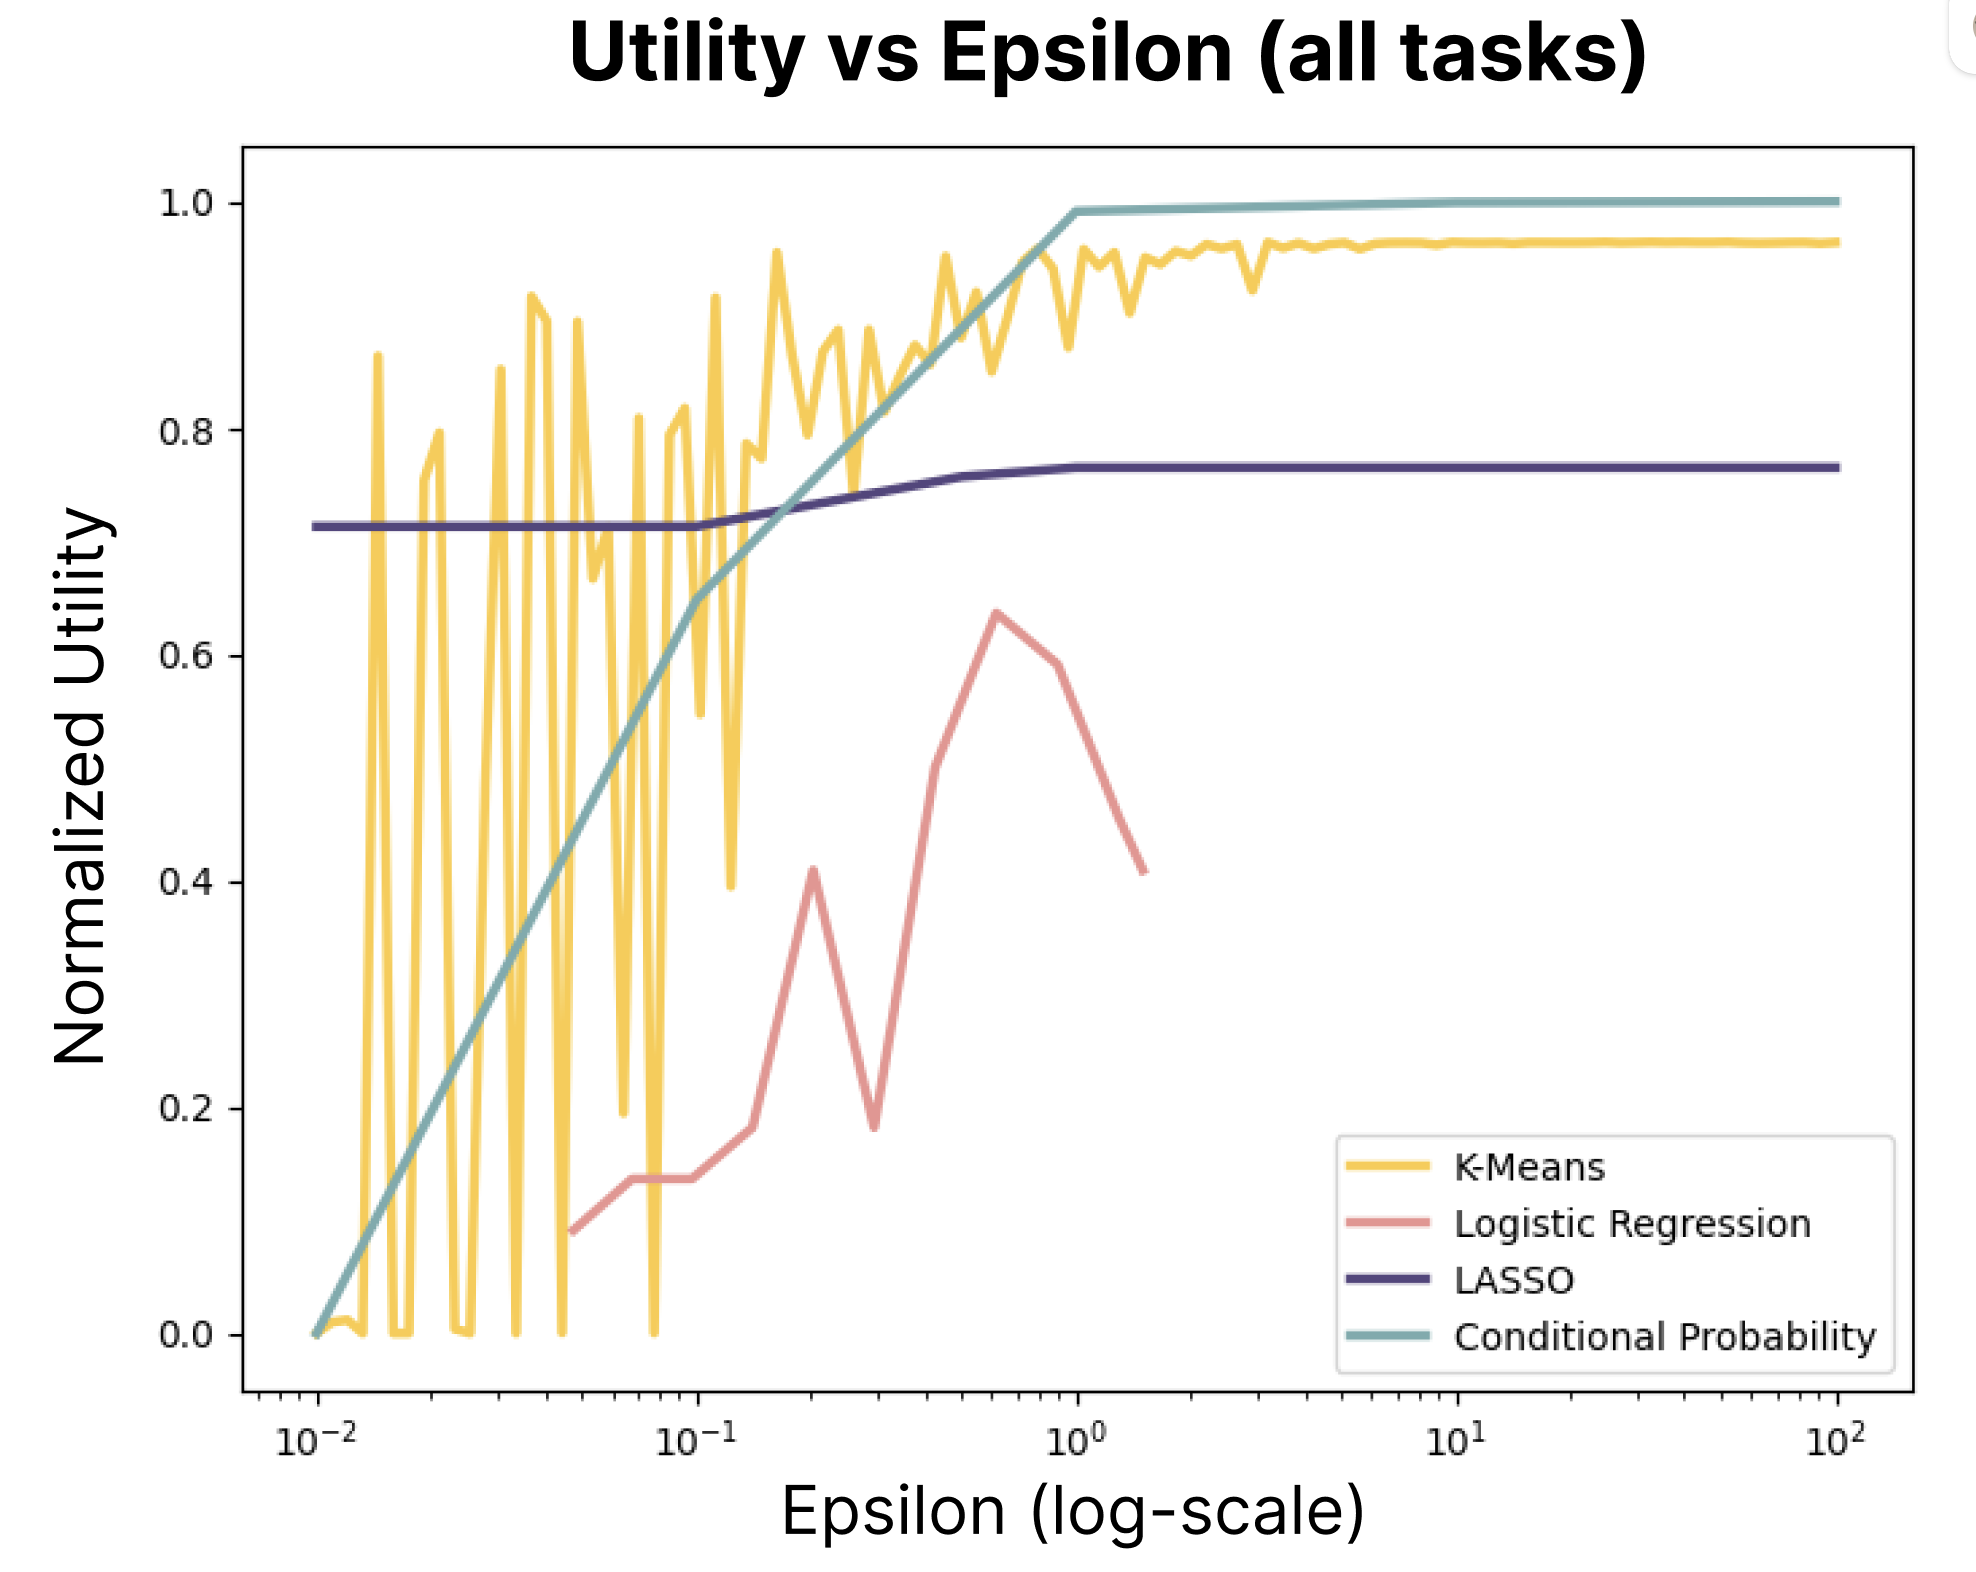
\includegraphics[width=0.6\textwidth]{figure/meta.png}
  \caption{Comparative Utility Analysis Across Privacy Budget ($\epsilon$) Levels. Non-private baselines for each task determines the maximum utility.}
  \label{fig:meta}
\end{figure}

\subsection{COND\_PROB}

Figure \ref{fig:histoeps} compares differences in private and non-private release of proportions for two error codes. Privacy budget total for this task was set to $\epsilon=1$. Uncorrected errors are coded 41, corrected errors are coded 1001. 

\begin{figure}[H]
    \centering
    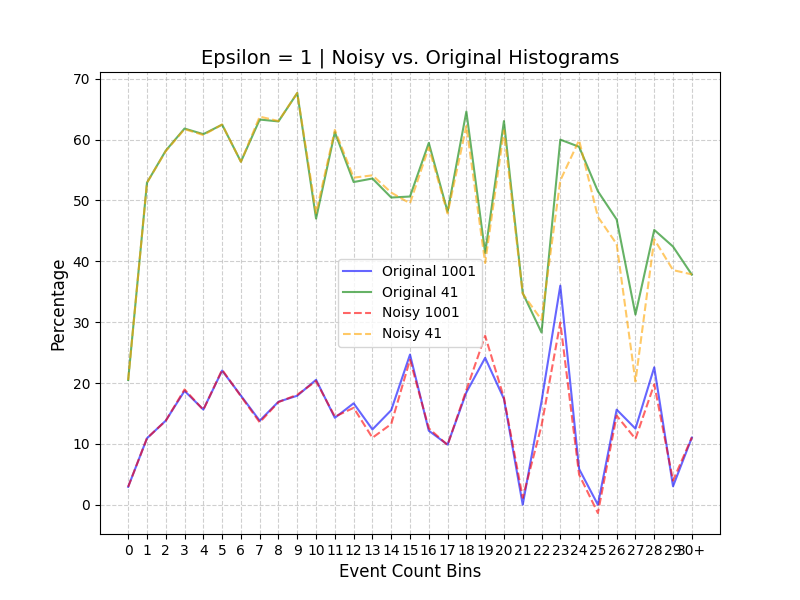
\includegraphics[width=0.8\textwidth]{figure/histoeps1.png}
    \caption{Corrected Error Count vs Uncorrected Error Probability at $\epsilon$ = 1 (with and without noise)}
    \label{fig:histoeps}
\end{figure}

Before transforming to utility, the conditional probabilities from Figure \ref{fig:histoeps} and releases at many other epsilons are measured in Mean Absolute Error. Figure \ref{fig:epsilon_vs_loss} shows a clear exponential decay even on log scaled epsilons, this indicates a super-exponential relationship between release error and budget. 

\begin{figure}[H]
    \centering
    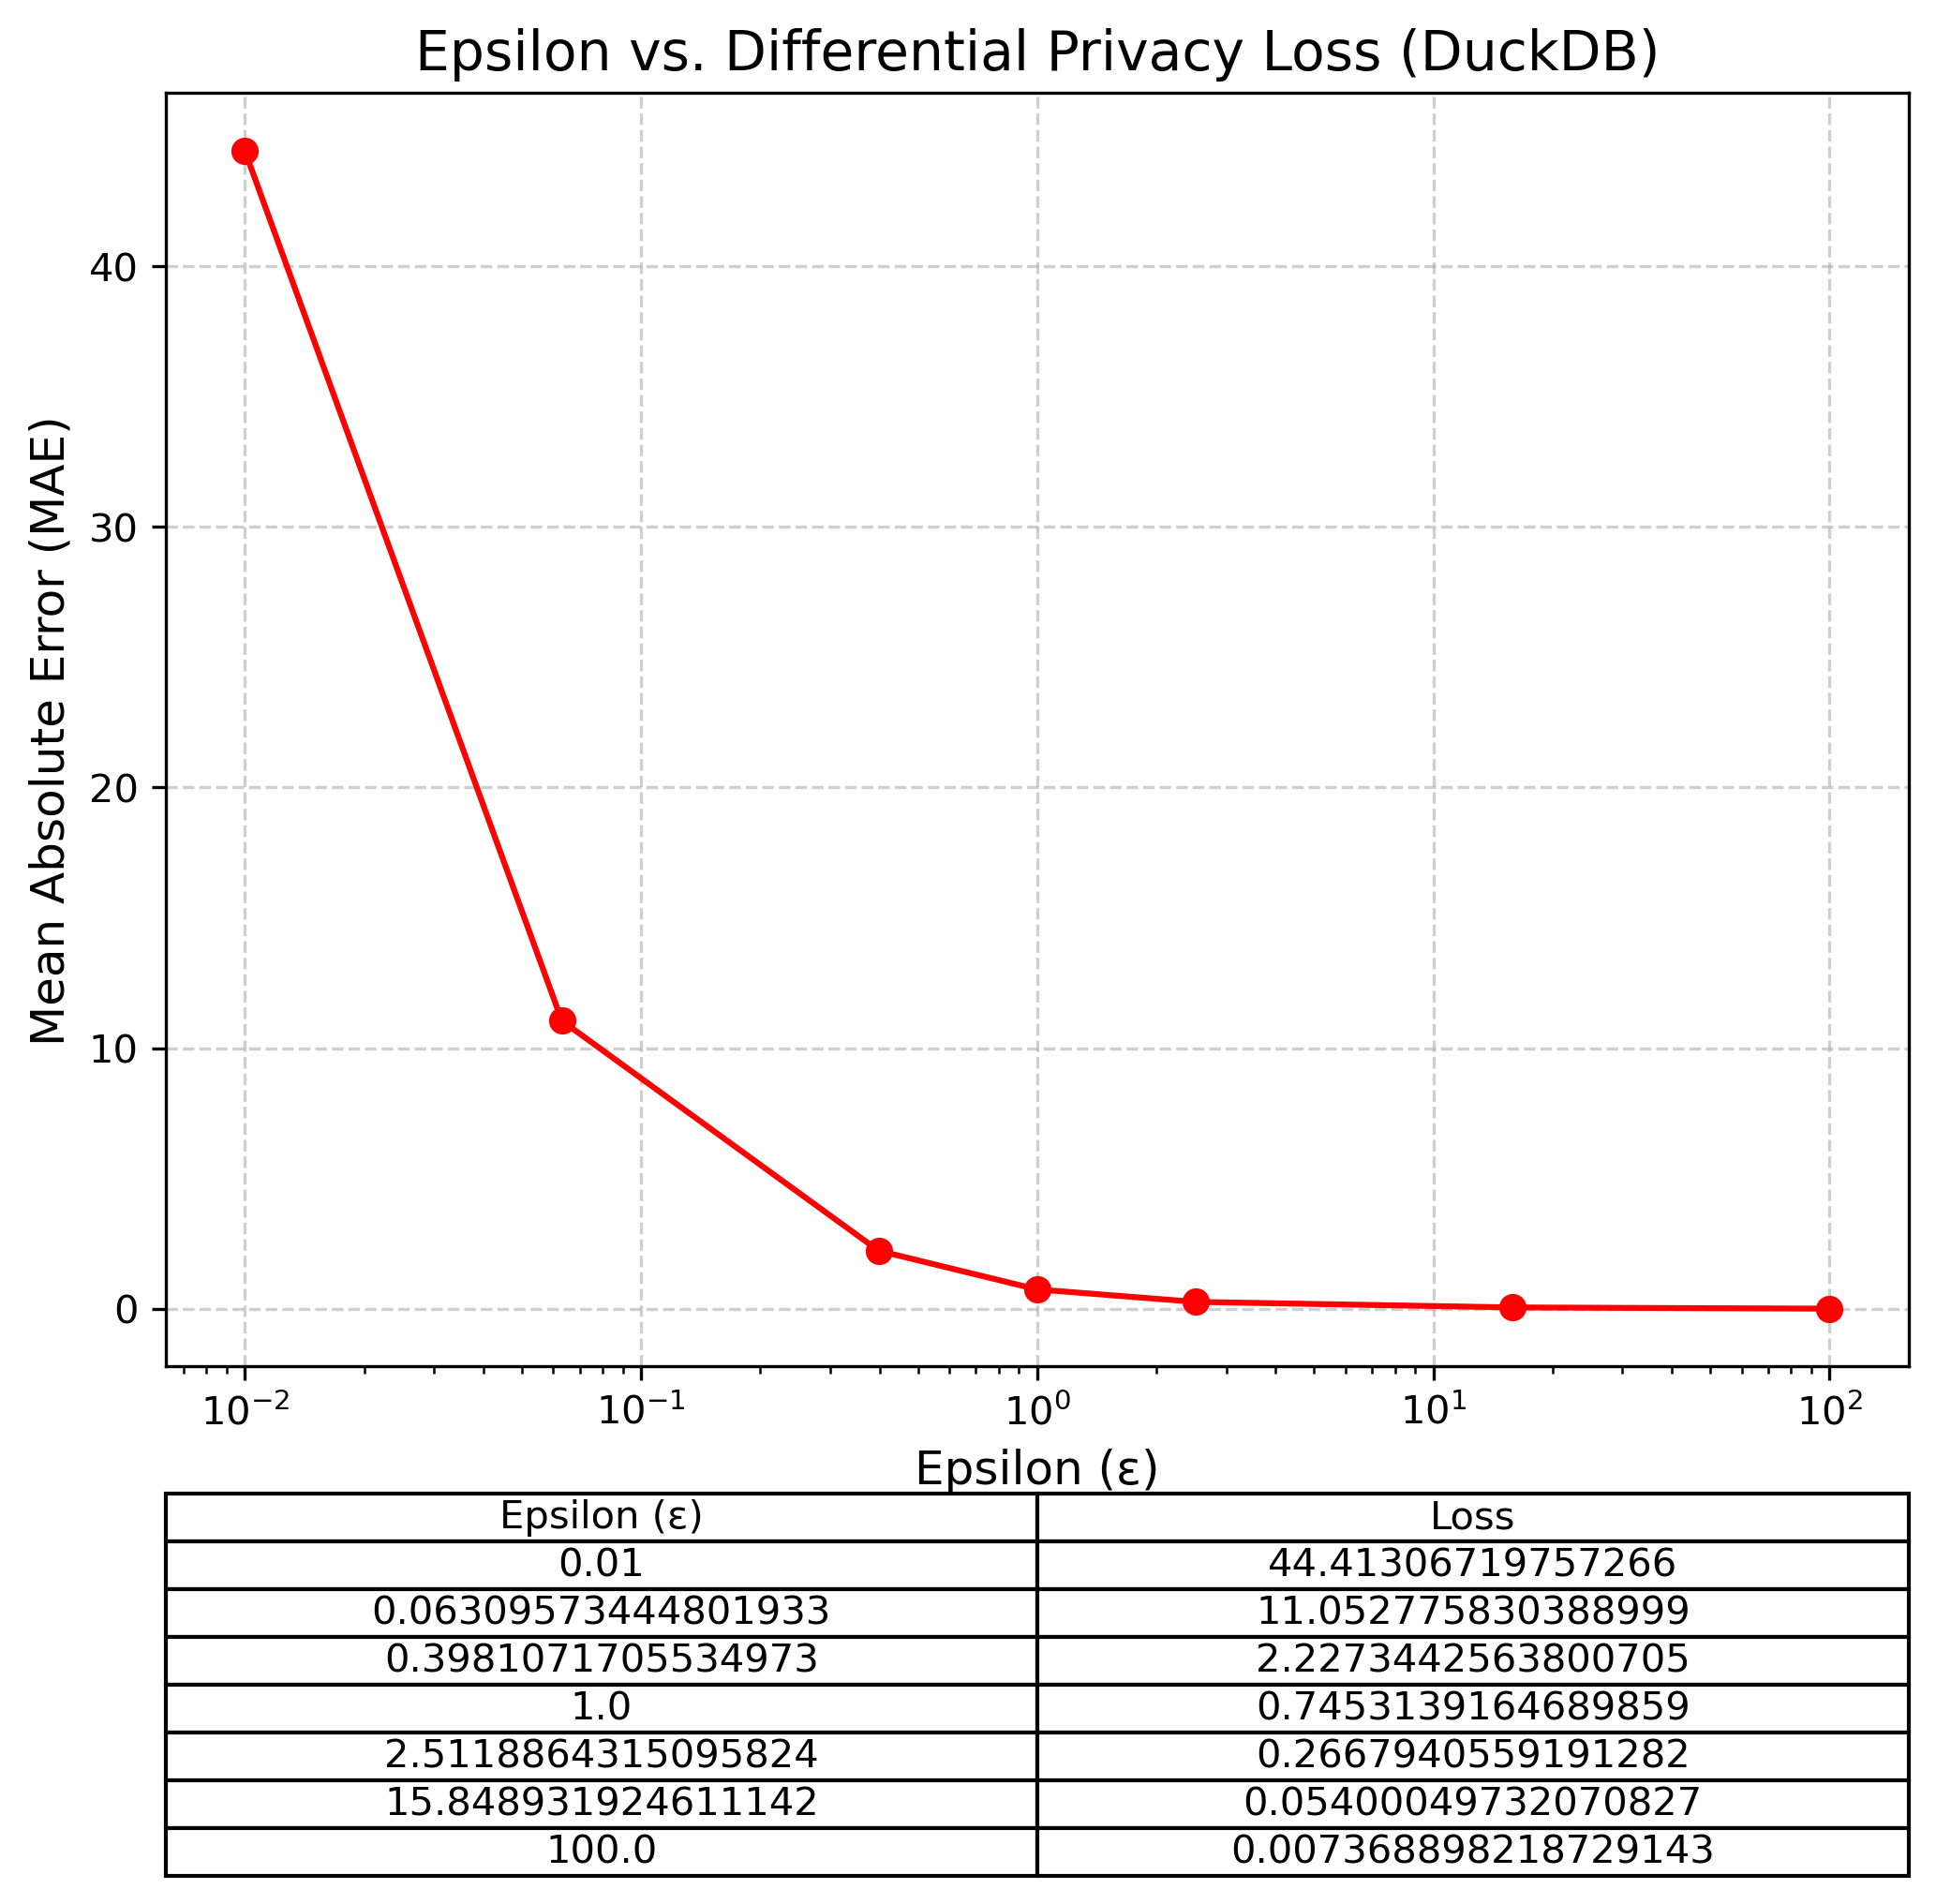
\includegraphics[width=0.8\textwidth]{figure/epsilon_vs_loss.png}
    \caption{Mean Absolute Error vs Epsilon}
    \label{fig:epsilon_vs_loss}
\end{figure}

\subsection{LR\_PVAL}
Our main method of comparing against the baseline was by calculating the set intersection over union for the private models and the non-private models. For epsilon = 1, the model severely under-shot the number of significant models. This means that it failed to find the correct relationship between corrected and uncorrected errors in a third (0.31) of the models.

\begin{figure}[H]
\centering
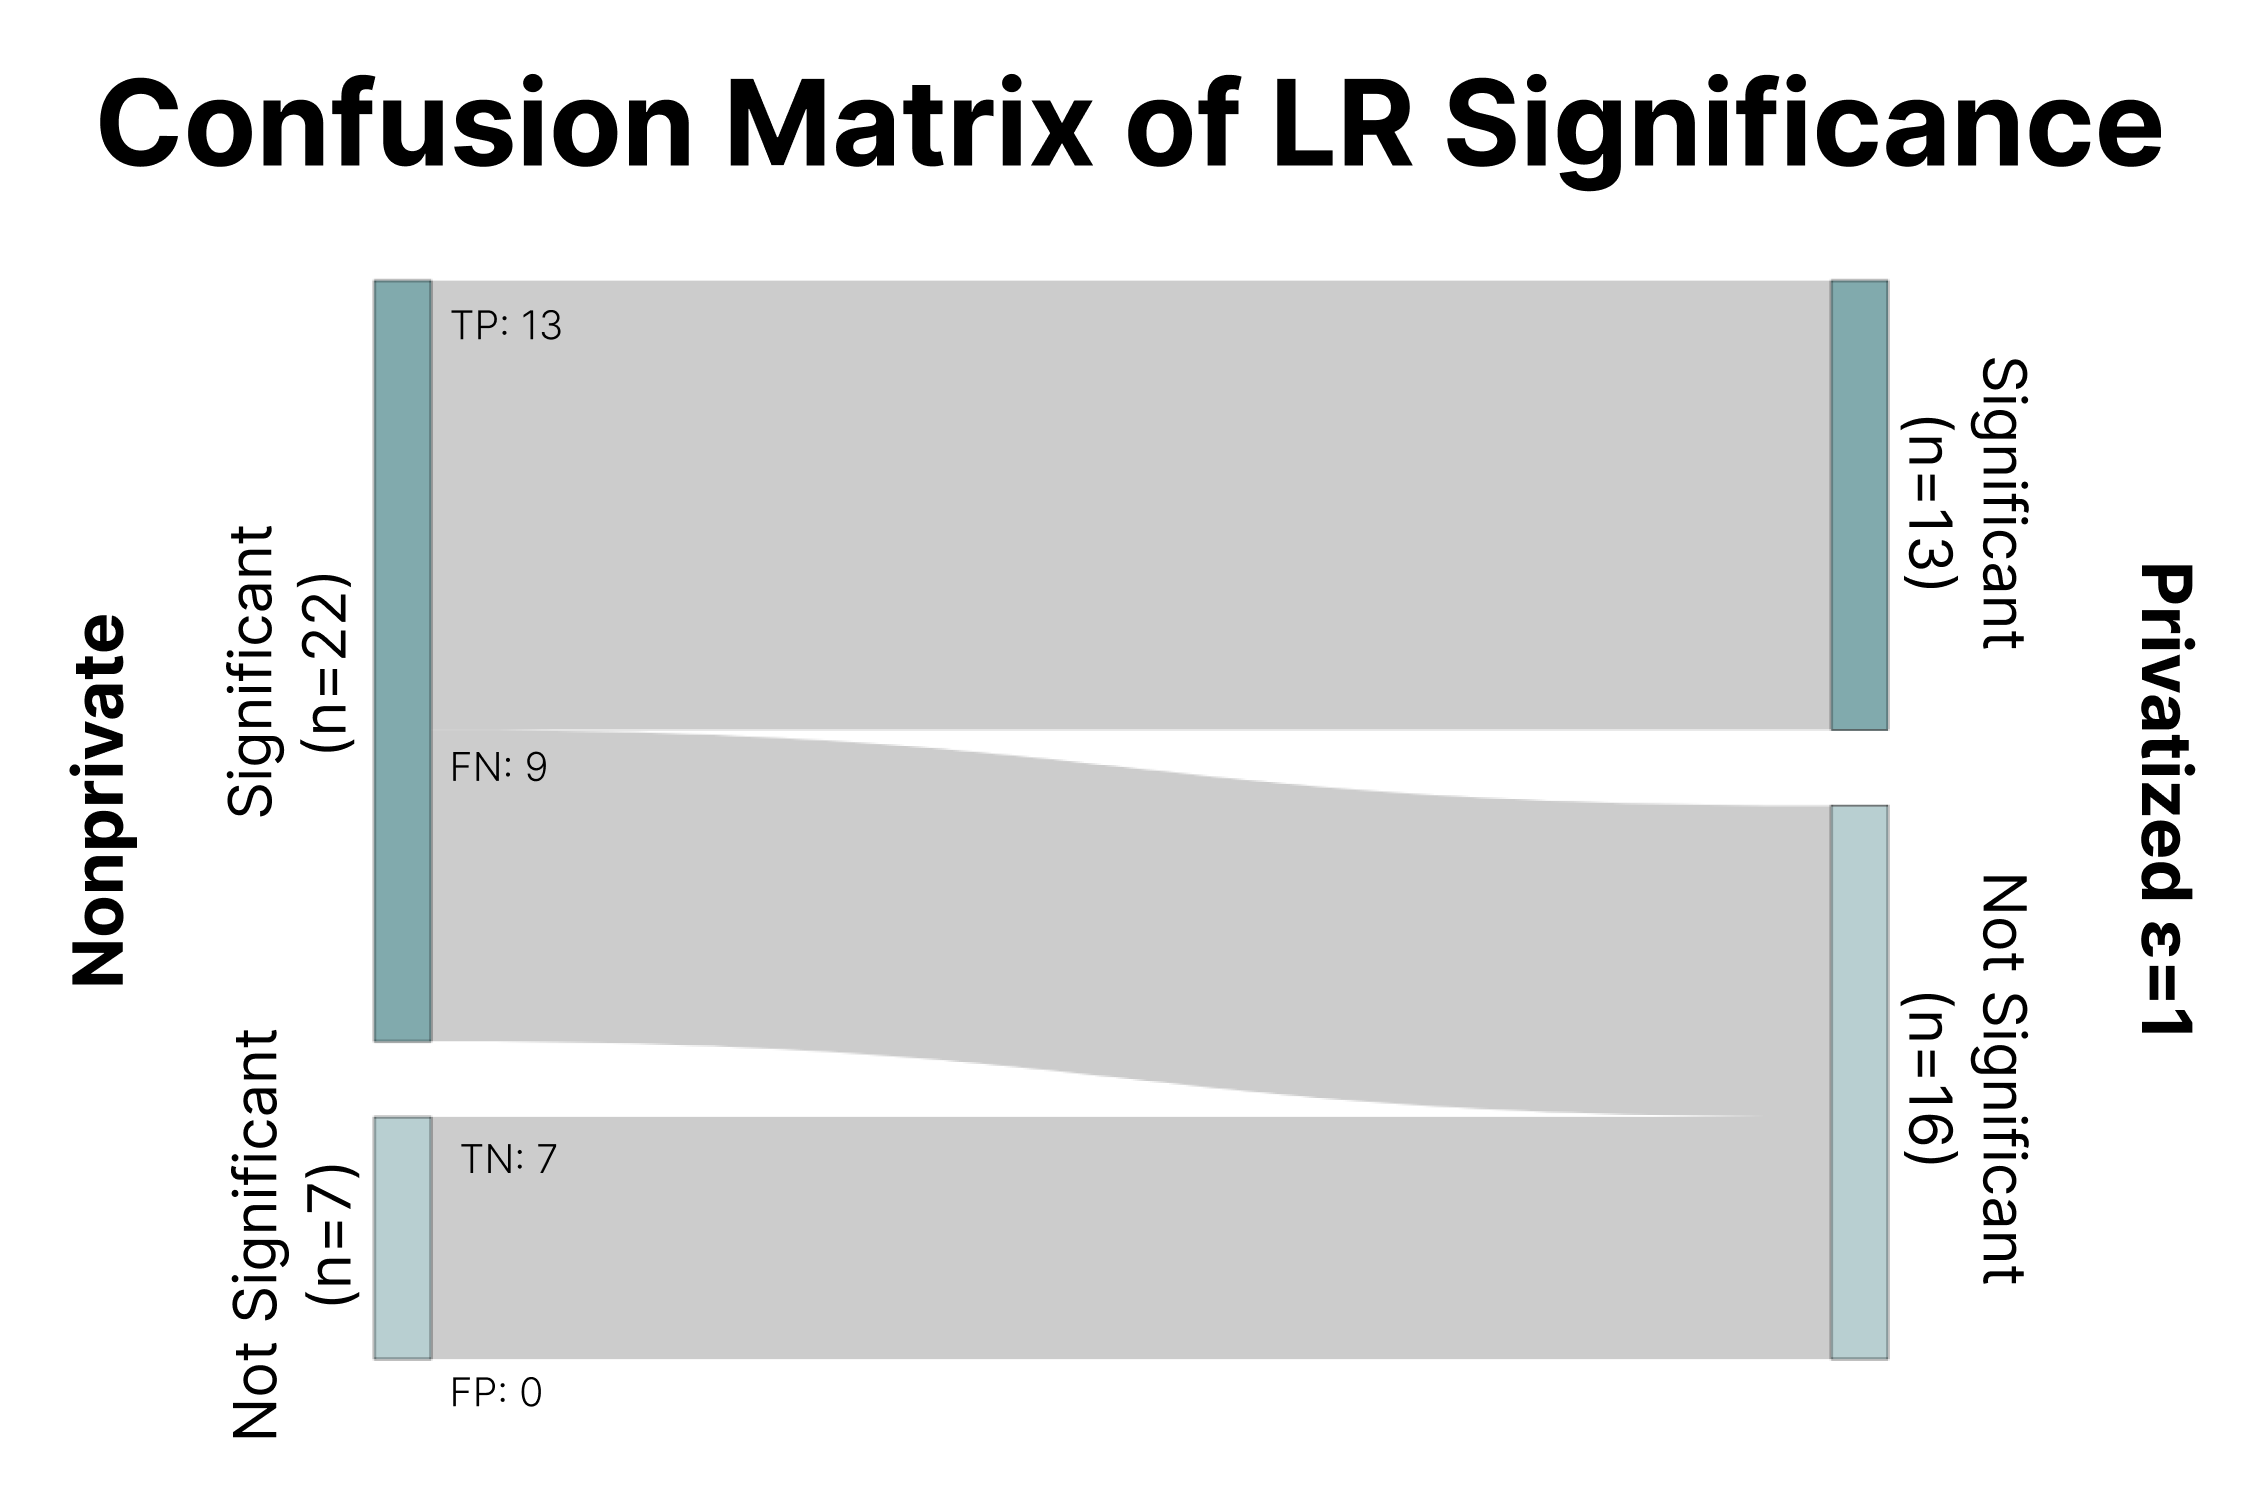
\includegraphics[width=.85\linewidth]{figure/conf_matrix.png}
\caption{Confusion matrix for $\epsilon$ = 1 for Wald Test. Right side has the private model classifications and the left has the non-private baselines. There were no false positives}
\label{fig:conf_matrix}
\end{figure}

\subsection{KMEANS}

Recreating the cluster visual from a previous study, in Figure \ref{fig:centroids} we display clusters of high dimensional data in terms of their scaled $L1$ Distance. There are three centers chosen for this model and they are spread in relation to data point densities.

\begin{figure}[H]
    \centering
    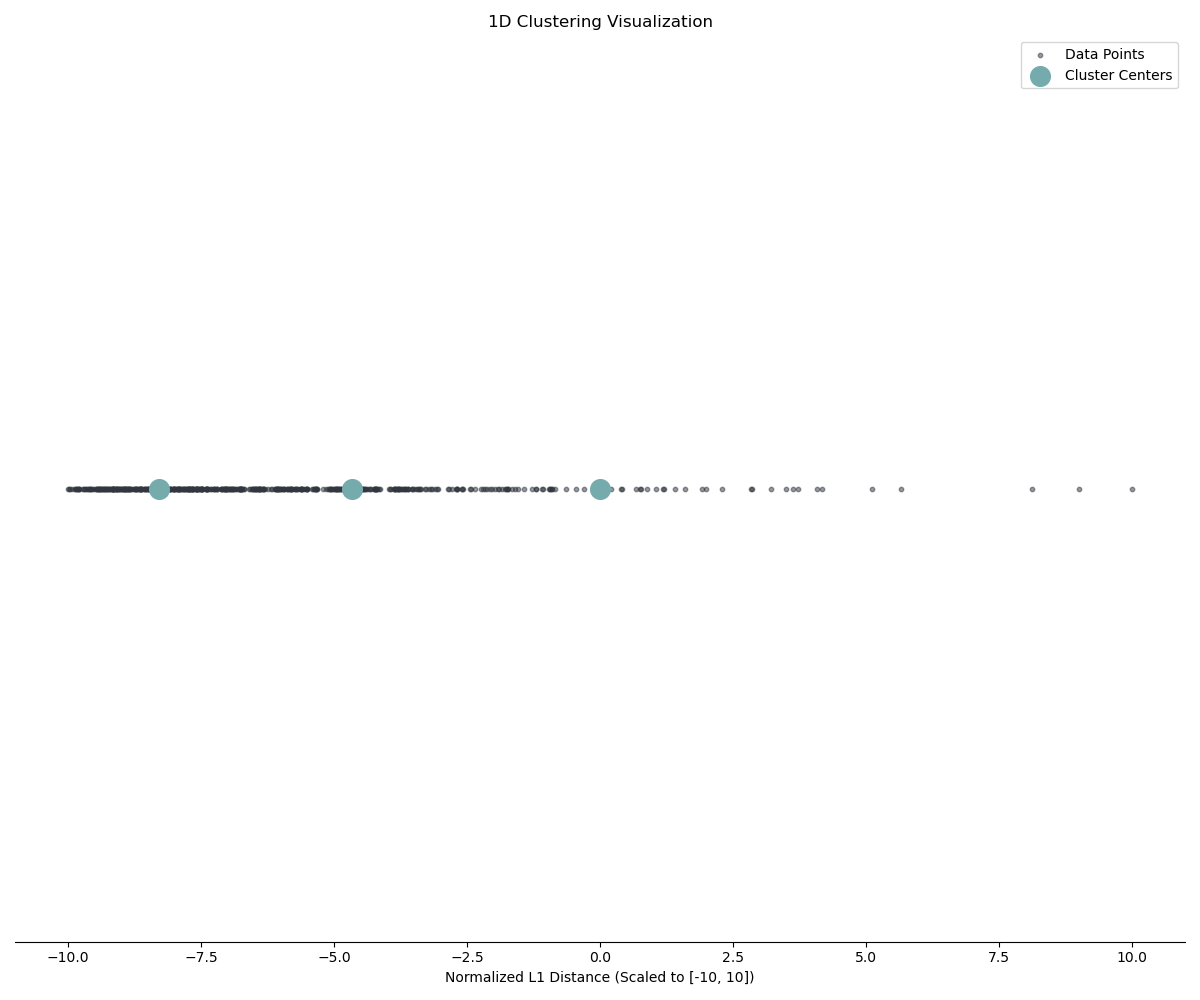
\includegraphics[width=0.6\textwidth]{figure/1d_clusters.png}
    \caption{Centroid locations overlaid over data points $\epsilon=1$}
    \label{fig:centroids}
\end{figure}

The model training evaluation at many privacy budgets is computed in Figure \ref{fig:epsilon_inertia}. Inertia measures total data spread from centroids and can fluctuate when any point is reassigned.

\begin{figure}[H]
    \centering
    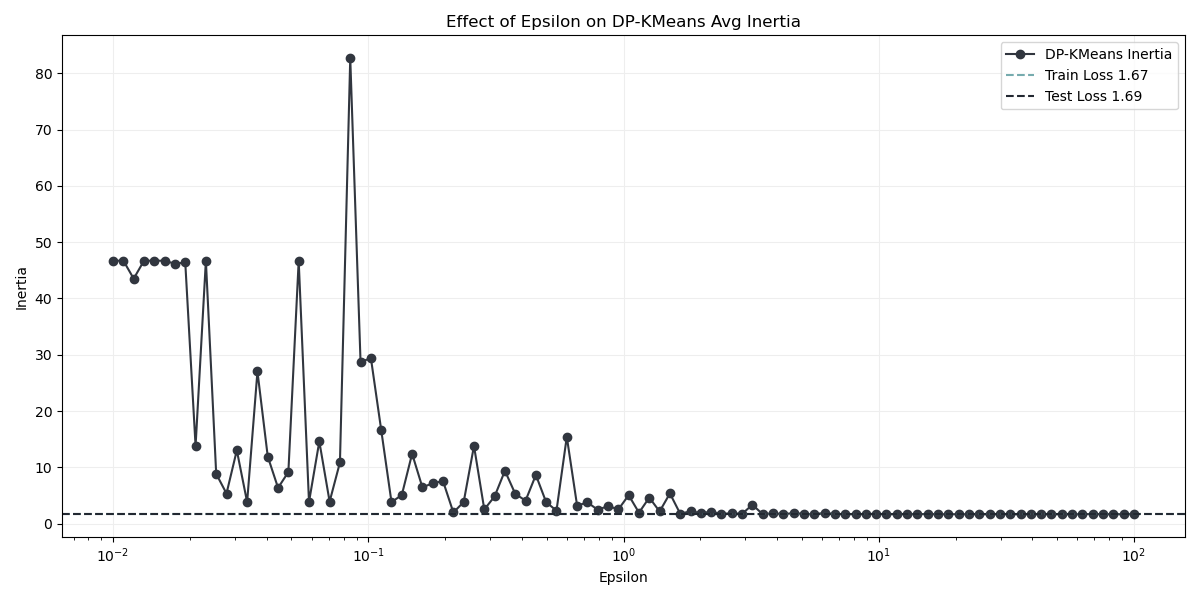
\includegraphics[width=0.6\textwidth]{figure/dpk_plot.png}
    \caption{Epsilon vs. Inertia compared to baseline non-private model}
    \label{fig:epsilon_inertia}
\end{figure}

\subsection{LASSO}

The power consumption driven carbon footprint paper trains a lasso model using typical coordinate descent and yields an RMSE of 5.86 (Watts) on the test set. Their correlation coefficient (R2) is 0.33.

Figure \ref{fig:lasso_convergence} shows convergence of the loss function to the optimal point for the non-private model, Frank-Wolfe lasso regression with exponential mechanism at many privacy levels. The regularization parameter $\lambda=10$ and total iterations $K=200$ are found from the results in Figure \ref{fig:lasso_results}.  

\begin{figure}[H]
    \centering
    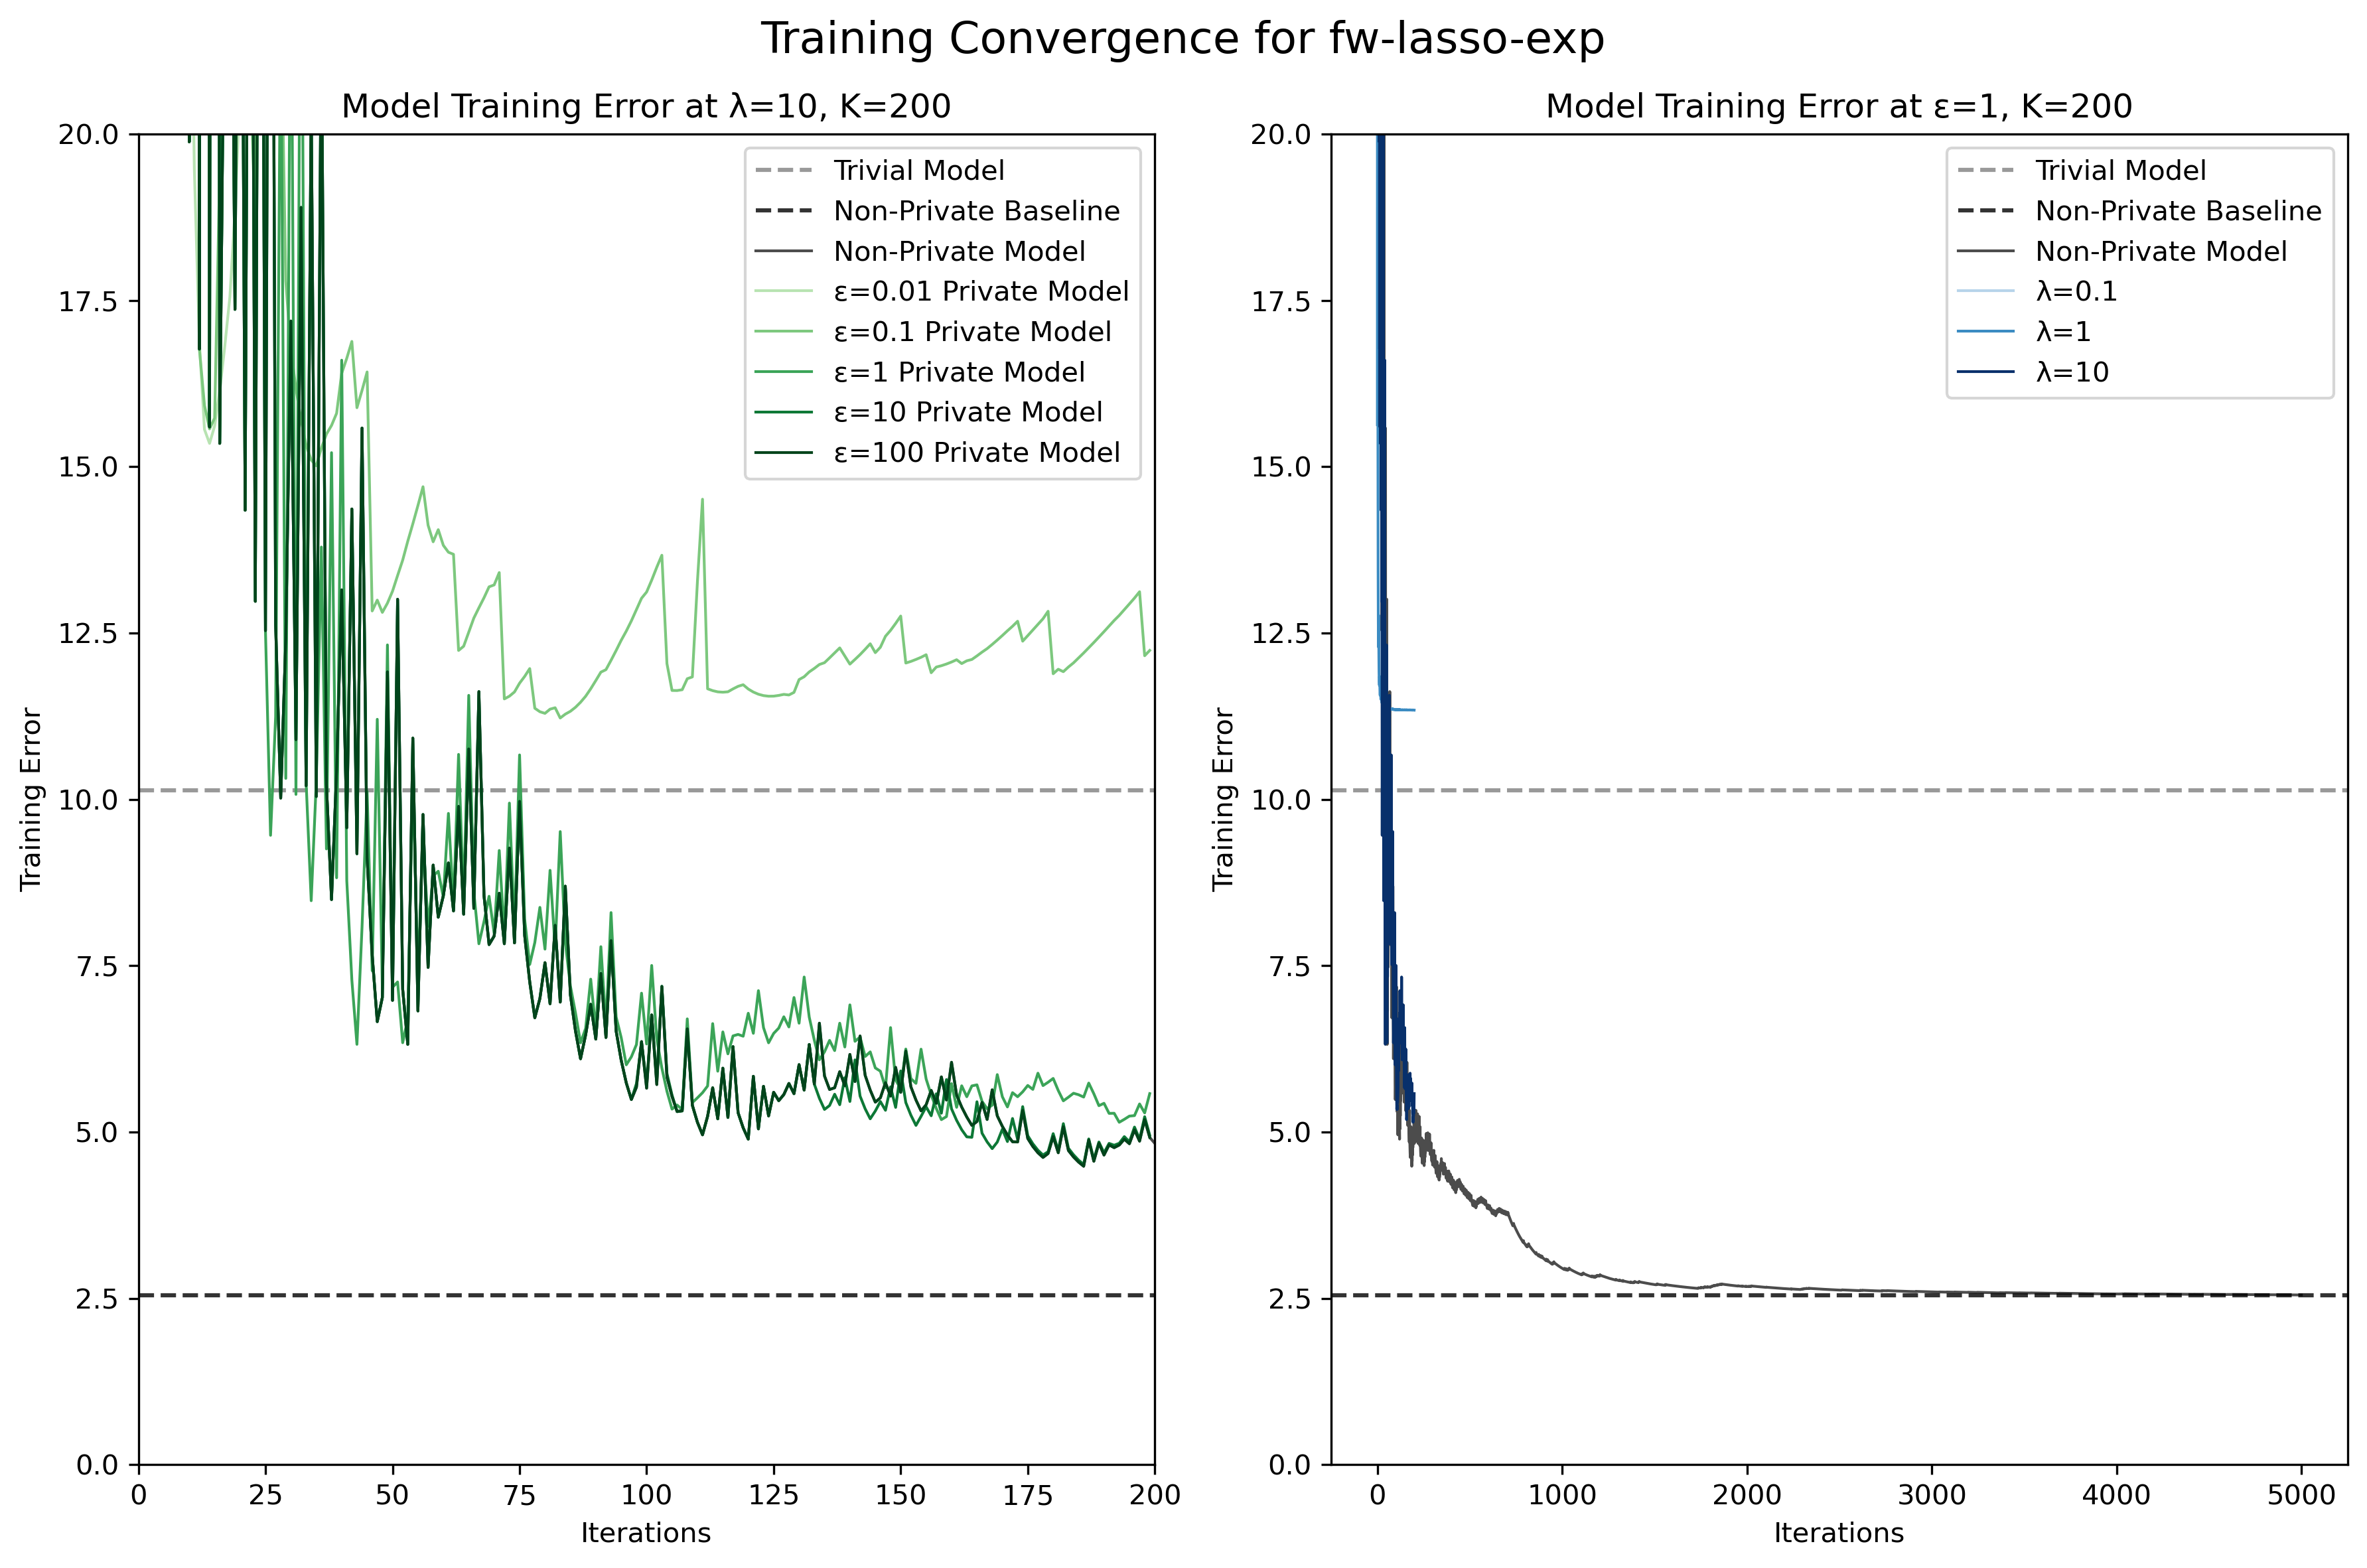
\includegraphics[width=0.9\textwidth]{figure/lasso_convergence.png}
    \caption{Convergence paths for various privacy budgets minimizing training error compared to non-private FW model.}
    \label{fig:lasso_convergence}
\end{figure}

The best baseline is found with $K=5000$ shown on the right. The private models are optimized at $K=200$, the $\epsilon=100$ model follows the same optimization path as non-private so the lines overlap, this is expected since almost no privacy is applied).

Figure \ref{fig:lasso_results} shows the performance of the models by viewing prediction error on a test set of data, the correlation coefficient R2, the similarity (0=none, 1=same features) found with the baseline Frank-Wolfe model, and the number of features that are kept in the solution.

\begin{figure}[H]
    \centering
    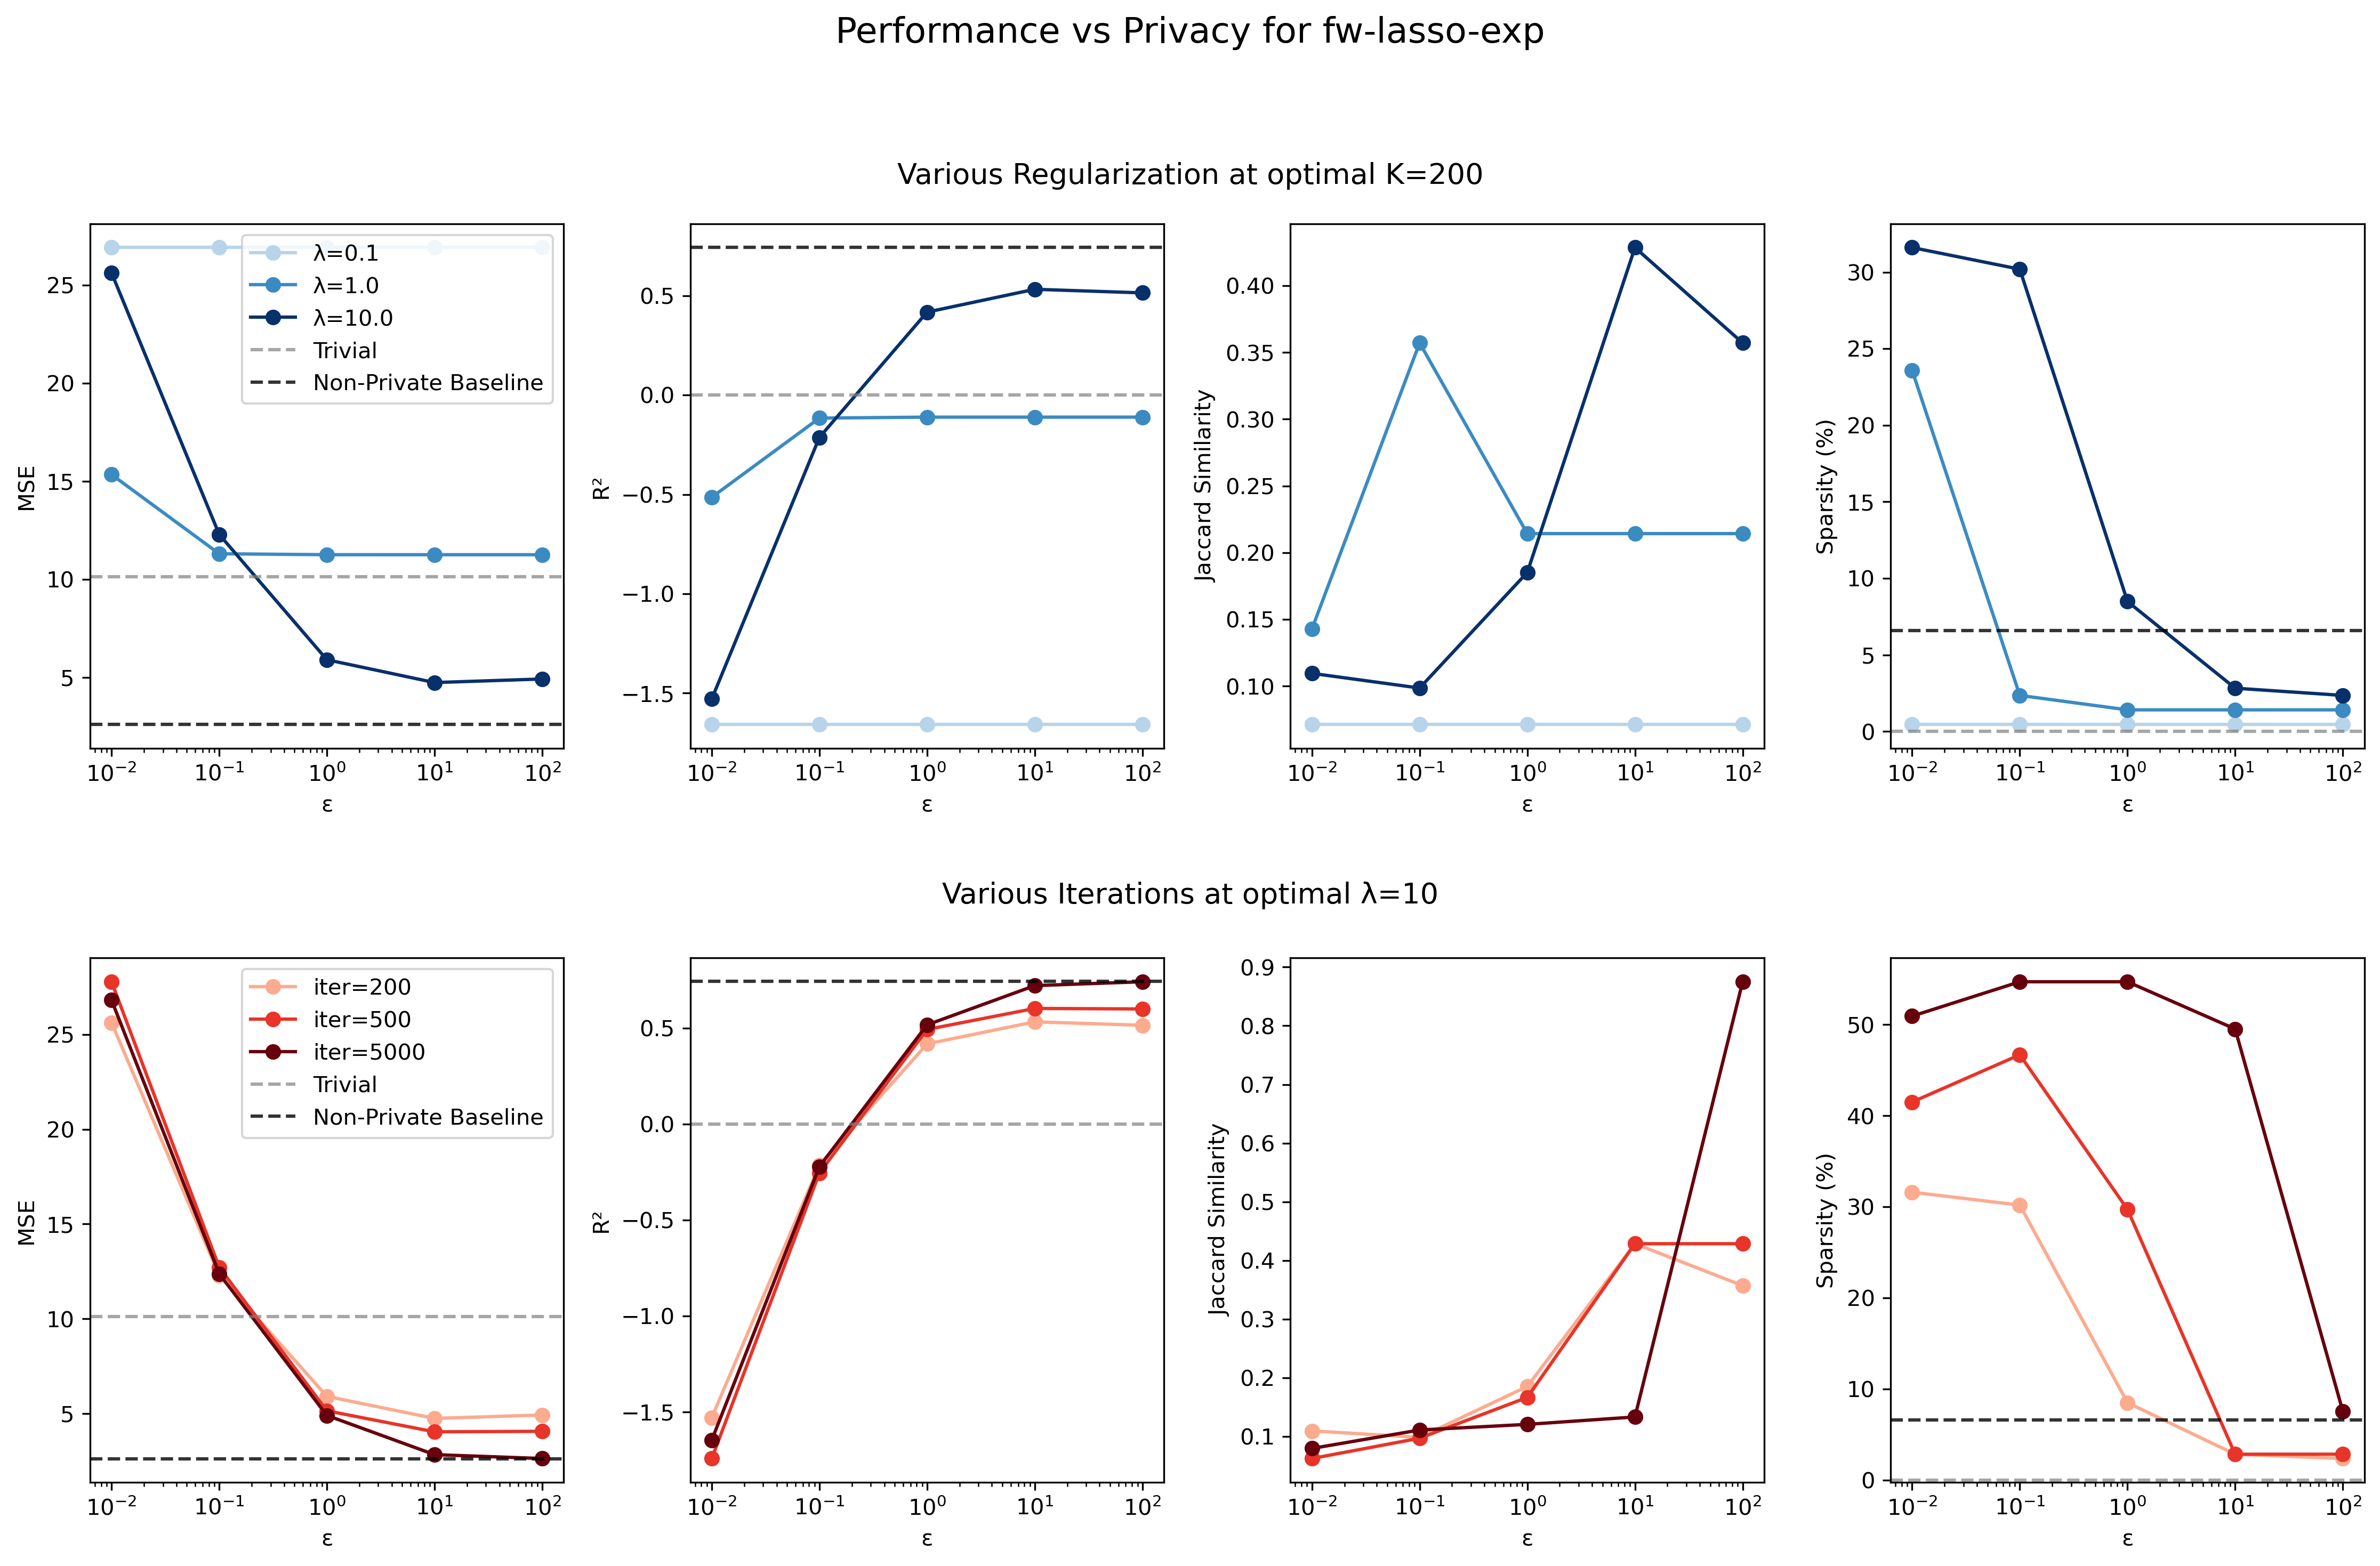
\includegraphics[width=0.95\textwidth]{figure/lasso_results.png}
    \caption{4 Performance metrics for various regularization ($\lambda$), privacy ($\epsilon$), and max iterations ($K$)}
    \label{fig:lasso_results}
\end{figure}

The Top row varies regularization $\lambda$ which is the penalty applied to the loss function; smaller lambda constrains the model more, resulting in more sparse solutions (column 4). The bottom row varies the number of iterations the algorithm is performed on, K=200 is the only viable solution since the sparsity as small as the non-private solution (at the target budget $\epsilon=1$).


%%%%%%%%%%%%%%%%%%%
%%%% DISCUSSION  %%%%%%%
%%%%%%%%%%%%%%%%%%%

\section{Discussion}


\subsection{Interpretation}
Our work provides a road map for integrating differential privacy into production environments, ensuring that sensitive telemetry data can be analyzed without compromising user privacy. This is particularly relevant for industries handling large volumes of user data. 

\subsubsection{Meta}
% BRADLEY %
For each task, the privacy-utility tradeoff is unique, conveying different sensitivities to noise. Some tasks can tolerate higher amounts of noise without significantly affecting the utility of the results, while others rely on precision and can degrade very fast with even slight noise. Given by our combined plot, each task has significantly different curves as epsilon changes. Added noise may reduce overfitting and could help the model generalize better, this is not an easy relationship to isolate for study. Some tasks were unable to reach non-private level utility even with large epsilon. Some required a minimum epsilon of > 0.1 to have utility above 50\%! We will analyze each individually as well.

\subsubsection{COND PROB}
Similar to established differential privacy theory and literature \cite{DworkRoth}, we observed a tradeoff between privacy and utility. However, our focus on conditional probability tasks allowed us to explore this tradeoff in a more specific context, providing insights into how differential privacy impacts analytical accuracy in this domain.

Our results show a significant increase in utility as ε increases. For instance, at ε = 0.1, the utility was approximately 0.65, which rose to nearly 0.99 at ε = 1 and reached almost 1 at ε = 100. This demonstrates that less stringent privacy guarantees (higher ε values) lead to higher utility.

For each epsilon, we found that as the number of corrected errors increased, the utility decreased. This is because the distribution of number of corrected errors is very heavily skewed left. The error amount with the largest amount of unique GUIDs is 0. This trend continues; as the number of corrected errors increases, the number of GUIDs with that exact amount of corrected errors decreases. This means the utility of the function is bounded by the maximum number of errors included in the histogram. We bounded our largest bin to be at 30 and found that an epsilon of 1 gave a sufficient utility. If we wanted to use a stricter epsilon, we would need to reduce the maximum corrected error to maintain the same utility. 


\subsubsection{LR\_PVAL}
Due to high compute costs, we were only able to get up to epsilon 1.5 for each of the 29 models. As we expected, the utility would increase from very low epsilon but around ε = 0.5, it is unclear whether or not the utility would continue to increase. At ε = 1, the model does somewhat poorly as seen in \ref{fig:conf_matrix}. The model has an intersect over union of around 0.60 and notably identifies a majority of the models as not significant, a result contrary to the nonprivate model. Overall, this analysis task did not seem to be replicable privately, at least under the strict privacy constraints.

It is important to note that this analysis would not be nearly as computationally hungry if we weren't trying to compare the models to a non-private model. In the practical setting, we wouldn't need to do permutation testing to find our p-values empirically. Similarly to the non-private setting, our alpha would be a hyperparameter that we would be able to select ourselves. This means that we may be able to use much higher values of epsilon in practice

\subsubsection{KMEANS}
The clustering algorithm is unsupervised so the best way to quantify performance is using inertia. It is the squared differences between data points and their nearest centroid. The smaller this value is, the better performing the cluster locations are, and therefore the model. 

As you can see from figure \ref{fig:centroids}, the cluster locations are located where the most data points are. Given that the distribution of the data is right skewed, it makes sense that the centroids, or cluster locations, are also right skewed to follow the data. 

From the figure \ref{fig:epsilon_inertia}, we can see that as epsilon increases, the inertia for the privatized model slowly converges to the non-private train and test loss. This is expected, and given its convergence close to an epsilon of 1, the model performs quite well in terms of both privacy and accuracy.

\subsubsection{LASSO}

The RMSE estimates the average amount each prediction is off of the truth by. We know 5 Watts is about $\frac{1}{10}$ the total power for a U-Series CPU, therefore, predictions are reasonable. The correlation coefficient then claims that R2\% of the variation in the dataset can be explained by the model features. The authors additionally state that given many possible factors are not included in the telemetry data, 33\% is a strong result.

Our results find an RMSE of 1.6 Watts for the Frank-Wolfe baseline algorithm and 2.28 Watts for the privatized at $\epsilon=1$, which is better performance than the original work. We see that the new baseline for explained portion of variance increased to 70\% by using Frank-Wolfe, and our private model is behind that at 50\%. The sparsity of chosen features is held at a manageable number by choosing a good K during training, there is no inherent benefit to having a couple more or less features between the private and non-private model (18 of 212 features were in the solution). The coordinate descent algorithm did not produce an identical baseline as the original paper, so other replication issues may exist that cannot be determined, this is why a new baseline is used.

The Jaccard similarity measures how similar the feature sets are that the private model found compared to the non-private. For most values below 0.4 for similar sized sets (sparsity condition), indicates remaining features are mostly different. This means the features Intel should improve first are different! This highlights a limitation of lasso as a means for finding causes; minimizing prediction error can generalize to test sets but with very different conclusions. There is no way to know which set has better chosen features, when additional tests are check to compare with the study’s original coordinate descent lasso, all the private and non-private Frank-Wolfe solutions had below 0.3 similarity furthering this point.

In totality, the private model had comparable test set error, and strong correlation which indicates a well fitted model. We postulate that the private lasso regression model is equally as informational and useful to Intel for their goal of reducing carbon emissions through targeted developments.


\subsection{Reflecting On The Process}
% CHRIS %
A part of assessing the feasibility of applying differential privacy is necessarily going to be a discussion surrounding the process of applying DP itself. We discuss what went well, what went poorly, and what limitations we had to concede.

\subsubsection{What was helpful}
% CHRIS %
In the process of applying differential privacy, we found three main things the most helpful: mathematical foundations of DP result in a consistent comparison across methods, differential privacy algorithms are intuitive at a high level, and that many papers exist on different DP algorithms ready to be implemented.

Comparing across methods was made easy because of the grounded-ness of DP in its definition and its reliance on epsilon. We could easily compare across tasks and observe that some tasks work well with an epsilon of 1 and some tasks didn't. The structure enabled us to have a strong idea that each of our privacy guarantees were identical.

Research therefore primarily focuses on theory, but we found that at a high level, DP algorithms are intuitive and straight forward. DP algorithms require three main ingredients: noise/randomness, bounded sensitivity, and privacy accounting. Determining noise scale, or what to clip and the best budgeting regime is tough, but each algorithm can be boiled down to those three.

Many traditional analysis tasks have been privatized and written about. Applying differential privacy oneself often relies on finding a paper detailing the mechanism and molding it for your specific use case. Additionally, authors have been responsive over email communication about their methods. We note that several times have we found minor errors in papers which made applying the methods difficult or produced misleading results. Overall, the methods already existed, and we needed to implement them.  

\subsubsection{What was difficult}
% CHRIS %
In the process, we found two main difficulties that hindered our ability to complete our analysis tasks: interpreting epsilon and quantifying utility loss.

Epsilon, as a value in the differential privacy equation, is straightforward with how it compares two probabilities. The issue is what this really looks like in real life. It is hard to get an intuition for what an arbitrarily bad event is and at what probability that would occur. We may know that our epsilons are the same, but what protections does that practically assure us? We know that an epsilon of 10 is bad, but how bad is it really? Sure, $e^{10}$ is a massive value, but what is the probability that something terrible actually happens?

On the other hand, we sought to measure utility loss as compared to a baseline. This had a set of difficulties in its own right. For some analysis tasks, the non-private version may not be the ground truth. For example, a lot of deep learning models generalize better when noise is added during training. Establishing what the maximum utility should be is not well defined. Furthermore, at a given amount of utility, how do you interpret the loss. For example in \cite{qtr1proj}, the logistic regression models had an IOU near 0.60. If the baseline was 0.8 how much utility is lost? At a more abstract level, what if being 1\% off is the difference between 100 million and 99 million lives saved? It's difficult to have a good intuition of what exactly we are losing. Utility is not a consistent or fair metric either, that 1\% loss may come from incorrect predictions only on data from minority demographics, or other biased results. With a restrained privacy budget, testing these results can be costly as well.

\subsubsection{Limitations}
% CHRIS %
There were a couple of limitations surrounding our ability to forge our analyses: missing background knowledge and replication vs. novel analysis.

Six months ago, differential privacy was a new concept to each of us. None of our backgrounds delved greatly into the rigor of mathematical proofs. Telemetry data was new to us and we suffered from lack of domain knowledge. Researchers or analysts who wish to accomplish similar comparisons may benefit greatly from more knowledge in either differential privacy and/or the domain in question itself. 

The applicability of our study as a commentary of the feasibility of DP methods must be framed knowing that we replicated existing research. Having the guidance of the original paper meant that there were some steps that we did not attempt or do privately ourselves. We did not try to tune hyperparameters privately, a task that would rely on high amounts of domain knowledge or using some of the privacy budget in order to find omptimal configurations. Further, we knew what features we wanted, private EDA is an entire privacy problem itself. One could argue that the analyst implementing a DP algorithm is already private and need not consider privacy in their analysis, but then the question arises, whom are we protecting against?

Replicating papers contains many of its own challenges. Obscurity in their writing, or lack of information about methods and data used leads to guessing. A common pitfall was not knowing exactly which "temperature" a paper was referring to. One of us had to assess several papers before being able to find one that would be replicable.


\subsection{The State of Differential Privacy}
The field of differential privacy is rapidly growing as more organizations and governments recognize the importance of protecting individuals' data in an increasingly data-driven world. It is crucial to be knowledgeable about this field as it equips us with the understanding of how to protect sensitive data while enabling meaningful analysis. Therefore it can be difficult to ensure your implementation has the best method, best budget and best interpretation for your task. Fortunately, even if your formulation is outdated, the guarantees will still hold and you will only be missing some marginal utility. 

%%%%%%%%%%%%%%%%%%%
%%%% CONCLUSION %%%%%%%
%%%%%%%%%%%%%%%%%%%

\section{Conclusion}


\subsection{Summary}
% CHRIS %
Overall, we found mixed results on how feasible applying differential privacy was. Some tasks were hardly affected and others would result in much different conclusions. There seems to be no universal solution for applying DP in tasks, it is task dependent. Different tasks have different success criteria, different methods have varying levels of ability to be privatized.

The feasibility of applying differential privacy seems to rely heavily on the practitioner's knowledge of both DP methods and their own domain. There is a high barrier to entry with differential privacy. An analyst who is familiar with their domain but completely new to DP would struggle greatly switching their workflow from their non-private methods to their private counterparts. Further, if the guarantees of DP aren't adequately understood, there would be a lack of desire in putting in the effort to lose utility and gain privacy. A path forward to private analyses across the board would not be able to be done bottom up, specialists would need to guide typical analysts.

\subsection{Impact}
% BRADLEY %
We recreated baseline models and algorithms used in previous research papers with their associated private models in a practical setting, providing valuable insights into how these privacy-preserving techniques perform in real-world applications. Our work demonstrates that with just a few months of practice and an understanding of differential privacy, it is possible to implement privacy-preserving methods that showcase the best epsilon that balances privacy and utility. As DP becomes even more accessible, it will make implementation faster, improving both performance and computation. Our code is open source, although the data is confidential, you may test our methods on your own datasets to see utility tradeoffs or use in practice.

\subsection{Future Direction}
% TYLER %
Future research could explore alternative differential privacy methods for our tasks, such as applying Lasso regression using the Functional Mechanism to improve utility while maintaining privacy. Additionally, investigating different privacy accounting regimes, such as Rényi differential privacy or zero-Concentrated DP, could provide a more flexible trade-off between privacy and accuracy, optimizing the overall performance of the model. 

Future work could focus on privatizing additional data tasks to enhance privacy while maintaining analytical utility. One potential task for future privatization is identifying the owning group for addressing a telemetry-detected issue, which could benefit from group-level differential privacy. This approach would help protect sensitive organizational information while still enabling efficient issue resolution. 

We could explore several directions to improve and expand differential privacy applications. One avenue is scaling up computations and applying privatization methods to different domains, enabling broader adoption in diverse fields such as gaming analytics, hardware performance, and behavioral studies. Additionally, investigating tasks with varying sensitivity levels could lead to more nuanced privacy strategies, where higher-sensitivity tasks receive stronger protections while lower-sensitivity tasks maintain higher utility.

Another promising direction is leveraging off-the-shelf differential privacy packages, such as Google's DP library or PySyft, to streamline implementation and improve accessibility. This could facilitate the more widespread adoption and standardization of privacy-preserving methods.

Beyond technical advancements, think-aloud studies and longitudinal research could provide valuable insights into how users interact with differentially private systems in real-world settings. By observing users over time, we can refine privacy mechanisms to better align with practical workflows. Finally, validating utility results through alternative testing methods would help ensure that privacy-preserving models maintain effectiveness across different evaluation metrics, strengthening confidence in their real-world applicability


\subsection{Acknowledgments}

We would like to recognize the support of our instructor, Yu-Xiang Wang, for his guidance and feedback throughout the project. We would also like to thank the teaching staff Umesh Bellur and Shriniwas Kulkarni for their support and feedback. The tasks database was a foundational part of our work and was created by another student researcher: Qiyu Li. We also attended a workshop called "Workshop on Defining Holistic Private Data Science for Practice" hosted by ENCORE at UC San Diego, which helped greatly with our broad understanding of the state of the field of differential privacy in practice.

We also would like to thank the authors of the papers we referenced in our literature review. Their work was instrumental in our understanding of the topic and the development of our project. Our understandings of differential privacy has been built on the work of many researchers in the field. Especially those which engaged in discussion with us about the field (Smith, Ulman, Kamath and others). We are grateful for their passion and for making their work freely accessible.

% COMMENT THIS BEFORE RENDERING
%\input{example_tex_section_6.tex}
% COMMENT THIS BEFORE RENDERING

%%%%%%%%%%%%%%%%%%%
%%%% REFERENCES%%%%%%%
%%%%%%%%%%%%%%%%%%%
\makereference

\bibliographystyle{style/dsc180bibstyle}


\bibliography{reference}
% To edit the contents of the ``References" section, edit \texttt{reference.bib}. Many conference websites format citations in BibTeX that you can copy into \texttt{reference.bib} directly; you can also search for the paper on Google Scholar, click ``Cite", and then click ``BibTeX" (\href{https://scholar.google.com/scholar?hl=en&as_sdt=0%2C23&q=attention+is+all+you+need&btnG=#d=gs_cit&t=1700436667623&u=%2Fscholar%3Fq%3Dinfo%3A5Gohgn6QFikJ%3Ascholar.google.com%2F%26output%3Dcite%26scirp%3D0%26hl%3Den}{here}'s an example).


%%%%%%%%%%%%%%%%%%%%%%%%%%%%%%%%%%%%%%%%%%%%%%%%%%%%%%%%
%%%% Appendix
%%%%%%%%%%%%%%%%%%%%%%%%%%%%%%%%%%%%%%%%%%%%%%%%%%%%%%%%

\clearpage
\makeappendix

%%%%%%%%%%%%%%%%%%%%%%
%%%% CONTRIBUTIONS %%%
%%%%%%%%%%%%%%%%%%%%%%

\subsection{Contributions}

\subsubsection{Author Contributions}
T.S. focused on lasso regression to highlight the exploratory capabilities of private data while implementing a previously theoretical framework (private Franke-Wolfe \cite{NIPS2015_52d080a3}). C.L. focused on private logistic regression to be able to do Wald tests to asses the relationship between input and target variables. B.N. analyzed and implemented non-private and private K-Means clustering. T.K. analyzed the experimental results of applying privacy mechanisms to a conditional probability histogram. Y.W. supervised the research and provided guidance on the mathematical foundations. All authors contributed to writing and reviewing the manuscript.

\subsubsection{Task Details}

Trey Scheid
\begin{itemize}
    \item Replication of \cite{lassocarbon}
    \item Implementation of non-private franke-wolfe lasso regression
    \item Ethical considerations of methods and impact
    \item Implementation of private franke-wolfe lasso regression
\end{itemize}

Tyler Kurpanek
\begin{itemize}
    \item Replication of Exploration of CPU Error Dependencies and Prediction \cite{Kwasnick2023}
    \item Implementation of Laplace Mechanism 
\end{itemize}

Bradley Nathanson
\begin{itemize}
    \item Replication of k-means clustering with Lloyd's algorithm \cite{kmeans}
    \item Implementation of privatized k-means clustering
\end{itemize}

Christopher Lum
\begin{itemize}
  \item Preprocess and replicate logistic regression paper privately and non-privately \cite{prodhealLR}
  \item Develop website
\end{itemize}

Yu-Xiang Wang
\begin{itemize}
  \item Concept ideation
  \item Data Access (Intel-HDSI research partnership)
  \item Provided guidance on the mathematical foundations
  \item Proofing and editing all content
\end{itemize}


\subsection{Project Proposal}

\textit{Proposed in coordination with mentor Yu-Xiang to the capstone faculty on 04 December, 2024.}

% style bad
% % !TEX TS-program = xelatex
% !BIB TS-program = bibtex
\documentclass[12pt,letterpaper]{article}
\usepackage{style/dsc180reportstyle} % import dsc180reportstyle.sty

%%%%%%%%%%%%%%%%%%%%%%%%%%%%%%%%%%%%%%%%%%%%%%%%%%%%%%%%
%%%% Title and Authors
%%%%%%%%%%%%%%%%%%%%%%%%%%%%%%%%%%%%%%%%%%%%%%%%%%%%%%%%

\title{DSC Quarter 2 Capstone Project Proposal}

\author{Bradley Nathanson \\
  {\tt bnathanson@ucsd.edu} \\\And
  Christopher Lum \\
  {\tt cslum@ucsd.edu} \\\And
  Trey Scheid \\
  {\tt tscheid@ucsd.edu} \\\And
  Tyler Kurpanek \\
  {\tt tkurpane@ucsd.edu} \\\And
  Yu-Xiang Wang \\
  {\tt yuxiangw@ucsd.edu} \\}

\begin{document}
\maketitle





\section{Proposal}
\subsection{Problem Statement}

Telemetry data is important to privatize as it encodes personally identifiable information which could be used to discover sensitive information. This data is collected from various IT devices, from satellites to personal computers. For our project, the telemetry data includes hardware and software performance metrics, monitoring, and errors. 

We will privatize 22 analysis tasks for the Intel telemetry dataset, ensuring a reasonable privacy budget (). We will implement mechanisms that balance data utility and privacy, ensuring sensitive information is protected, and allocate a reasonable privacy budget (), a parameter that governs the trade-off between accuracy and privacy.

One example of a task is to predict CPU failure. This would require a privatized logistic regression model that predicts the probability of a failure from 0-1. The model would analyze data such as CPU temperature, usage patterns, error logs, or other performance indicators. If non-privatized, this model could expose this data, as a malicious individual could do a reconstruction attack, a method to reconstruct the training data by repeatedly querying the model with various synthetic inputs. The attacker could query this model with different sets of CPU-related inputs, and, over time, the attacker could gain information such as the CPU temperature threshold for an error to occur, or whether certain system configurations have a distinct failure pattern.

\subsection{Methods}
Our methodology for privatizing the 22 telemetry analysis tasks will employ multiple privacy mechanisms, such as the exponential mechanism and the Laplace mechanism, with AutoDP serving as our core privacy accounting tool. For each analysis task, we will first evaluate the sensitivity of the computation and determine the optimal privacy mechanism to maintain utility while satisfying privacy requirements. The implementation process requires careful privacy budget allocation across multiple components of each analysis to ensure the total privacy loss remains within acceptable bounds.

The evaluation of each privatized implementation will involve a comprehensive comparison with non-private baselines to document the privacy-utility tradeoff. This includes analyzing performance metrics before and after applying privacy mechanisms, measuring accuracy degradation at various privacy budget levels, and considering computational efficiency challenges specific to telemetry data analysis. AutoDP will help quantify the privacy guarantees and guide the noise calibration process throughout implementation. 

Each privatized task will be thoroughly documented with implementation details, privacy guarantees, and performance metrics. This documentation will include privacy budget allocation strategies, noise mechanism selection rationale, and practical guidelines for future implementations. The goal is to create a comprehensive resource demonstrating how different privacy mechanisms can be effectively applied to various telemetry analysis scenarios while maintaining practical utility and ensuring strong privacy protections.


\subsection{Deliverable}
The privatized analysis tasks will be stored and shared in a public repository, (without release of source data from Intel). This is our primary contribution, to offer tools in a privatized manner. In collaboration with the accessible programs, we will publish a website that will serve to educate our peers on differential privacy. The variety of analysis tasks done in the telemetry domain can be generalized and applied to many types of data; therefore, descriptions of privacy algorithms, their motivations, and limitations can teach practitioners new methods for their own tasks. 

The Intel data as mentioned is not public (due to the customer privacy and proprietary nature). Therefore our data processing, tasks, and report will include only some metrics of performance and data quality (size, distribution, features, etc). For the information we can share, we will compare the performance of the task with that of the non-private baseline. This gives analysts a sense of the utility-privacy tradeoff in each application. 

\subsection{Impact}
By implementing differential privacy across telemetry we will create a significant impact by maintaining data confidentiality. This project will establish novel approaches to common tasks enabling hardware manufacturers to analyze system performance data while preserving strong privacy guarantees. This advances the field by demonstrating how to maintain data utility while protecting sensitive information in real-world applications. 

The research contribution includes documenting privacy-utility trade-offs and establishing guidelines for privacy budget allocation across multiple analysis tasks. Our work will demonstrate practical privacy considerations in telemetry analysis while protecting users’ participation in datasets. The methodologies developed can be adapted by other researchers working with sensitive telemetry data. 

\subsection{Success Criteria}
The success of this project is dependent on a few factors. The first two are team collaboration and schedule adherence. There are many tasks that can be privatized and there may be unique challenges for each (hence the value in sharing these!). With one-quarter complete with group work on our privatized logistic regression paper, our group is confident in our communication, task management, and problem-solving abilities. Paired with our mentor Yu-Xiang Wang, an expert in the field of differential privacy, and a seasoned professor, we are equipped to find innovative and theoretically founded methods for privatizing data tasks.

The other requirements for this project rely on data access and task availability. The Intel data is proprietary, and we have signed agreements to use the data for research, however strict access and usage terms have not been given to us yet. Previous students have worked with the contact/program at Intel successfully and we are reassured by them that we will have a usable telemetry dataset by the start of the quarter.  Similarly, there is a set of non-privatized tasks completed on this dataset by previous data scientists, their work is the foundation which we will build off of to show utility is possible even with privacy. These projects were successful implementations on the specific dataset we will have access to, this pairing therefore will continue to bear fruit as we privatize the tasks and compare baselines. 

Lastly, although we have not reviewed the dataset and tasks yet (no access), the intel program is sharing genuine telemetry information from devices with given consent as part of their program. Additionally, this HDSI-Intel partnership has been cooperating since 2020 and HDSI has used hundreds of terabytes of information. 





\end{document}

\subsubsection{Problem Statement}

Telemetry data is important to privatize as it encodes personally identifiable information which could be used to discover sensitive information. This data is collected from various IT devices, from satellites to personal computers. For our project, the telemetry data includes hardware and software performance metrics, monitoring, and errors. 

We will privatize 22 analysis tasks for the Intel telemetry dataset, ensuring a reasonable privacy budget (). We will implement mechanisms that balance data utility and privacy, ensuring sensitive information is protected, and allocate a reasonable privacy budget (), a parameter that governs the trade-off between accuracy and privacy.

One example of a task is to predict CPU failure. This would require a privatized logistic regression model that predicts the probability of a failure from 0-1. The model would analyze data such as CPU temperature, usage patterns, error logs, or other performance indicators. If non-privatized, this model could expose this data, as a malicious individual could do a reconstruction attack, a method to reconstruct the training data by repeatedly querying the model with various synthetic inputs. The attacker could query this model with different sets of CPU-related inputs, and, over time, the attacker could gain information such as the CPU temperature threshold for an error to occur, or whether certain system configurations have a distinct failure pattern.

\subsubsection{Methods}

Our methodology for privatizing the 22 telemetry analysis tasks will employ multiple privacy mechanisms, such as the exponential mechanism and the Laplace mechanism, with AutoDP serving as our core privacy accounting tool. For each analysis task, we will first evaluate the sensitivity of the computation and determine the optimal privacy mechanism to maintain utility while satisfying privacy requirements. The implementation process requires careful privacy budget allocation across multiple components of each analysis to ensure the total privacy loss remains within acceptable bounds.

The evaluation of each privatized implementation will involve a comprehensive comparison with non-private baselines to document the privacy-utility tradeoff. This includes analyzing performance metrics before and after applying privacy mechanisms, measuring accuracy degradation at various privacy budget levels, and considering computational efficiency challenges specific to telemetry data analysis. AutoDP will help quantify the privacy guarantees and guide the noise calibration process throughout implementation. 

Each privatized task will be thoroughly documented with implementation details, privacy guarantees, and performance metrics. This documentation will include privacy budget allocation strategies, noise mechanism selection rationale, and practical guidelines for future implementations. The goal is to create a comprehensive resource demonstrating how different privacy mechanisms can be effectively applied to various telemetry analysis scenarios while maintaining practical utility and ensuring strong privacy protections.


\subsubsection{Deliverable}

The privatized analysis tasks will be stored and shared in a public repository, (without release of source data from Intel). This is our primary contribution, to offer tools in a privatized manner. In collaboration with the accessible programs, we will publish a website that will serve to educate our peers on differential privacy. The variety of analysis tasks done in the telemetry domain can be generalized and applied to many types of data; therefore, descriptions of privacy algorithms, their motivations, and limitations can teach practitioners new methods for their own tasks. 

The Intel data as mentioned is not public (due to the customer privacy and proprietary nature). Therefore our data processing, tasks, and report will include only some metrics of performance and data quality (size, distribution, features, etc). For the information we can share, we will compare the performance of the task with that of the non-private baseline. This gives analysts a sense of the utility-privacy tradeoff in each application. 

\subsubsection{Impact}

By implementing differential privacy across telemetry we will create a significant impact by maintaining data confidentiality. This project will establish novel approaches to common tasks enabling hardware manufacturers to analyze system performance data while preserving strong privacy guarantees. This advances the field by demonstrating how to maintain data utility while protecting sensitive information in real-world applications. 

The research contribution includes documenting privacy-utility trade-offs and establishing guidelines for privacy budget allocation across multiple analysis tasks. Our work will demonstrate practical privacy considerations in telemetry analysis while protecting users’ participation in datasets. The methodologies developed can be adapted by other researchers working with sensitive telemetry data. 

\subsubsection{Success Criteria}

The success of this project is dependent on a few factors. The first two are team collaboration and schedule adherence. There are many tasks that can be privatized and there may be unique challenges for each (hence the value in sharing these!). With one-quarter complete with group work on our privatized logistic regression paper, our group is confident in our communication, task management, and problem-solving abilities. Paired with our mentor Yu-Xiang Wang, an expert in the field of differential privacy, and a seasoned professor, we are equipped to find innovative and theoretically founded methods for privatizing data tasks.

The other requirements for this project rely on data access and task availability. The Intel data is proprietary, and we have signed agreements to use the data for research, however strict access and usage terms have not been given to us yet. Previous students have worked with the contact/program at Intel successfully and we are reassured by them that we will have a usable telemetry dataset by the start of the quarter.  Similarly, there is a set of non-privatized tasks completed on this dataset by previous data scientists, their work is the foundation which we will build off of to show utility is possible even with privacy. These projects were successful implementations on the specific dataset we will have access to, this pairing therefore will continue to bear fruit as we privatize the tasks and compare baselines. 

Lastly, although we have not reviewed the dataset and tasks yet (no access), the intel program is sharing genuine telemetry information from devices with given consent as part of their program. Additionally, this HDSI-Intel partnership has been cooperating since 2020 and HDSI has used hundreds of terabytes of information.


\subsection{Additional Materials}

\subsubsection{Privacy Theorems and Definitions}

\begin{definition}[\cite{ExpMech} Exponential Mechanism]
    \label{def:ExpMech}
    Let $\mathcal{D}$ be a domain of datasets, $\mathcal{R}$ be a range of possible outputs, and $q: \mathcal{D} \times \mathcal{R} \rightarrow \mathbb{R}$ be a quality function that maps dataset-output pairs to real-valued scores. The sensitivity of $q$ is defined as:
    \[
    \Delta q = \max_{r \in \mathcal{R}, D, D' \text{ adjacent}} |q(D,r) - q(D',r)|
    \]
    
    The Exponential Mechanism $\mathcal{M}_q^{\epsilon}(D)$ selects and outputs an element $r \in \mathcal{R}$ with probability proportional to:
    \[
    \Pr[\mathcal{M}_q^{\epsilon}(D) = r] \propto \exp\left(\frac{\epsilon q(D,r)}{2\Delta q}\right)
    \]
    
    The Exponential Mechanism satisfies $\epsilon$-differential privacy. Furthermore, if we define $OPT(D) = \max_{r \in \mathcal{R}} q(D,r)$ as the maximum quality score, then with probability at least $1-\delta$:
    \[
    q(D, \mathcal{M}_q^{\epsilon}(D)) \geq OPT(D) - \frac{2\Delta q}{\epsilon}\left(\ln\left(\frac{|\mathcal{R}|}{\delta}\right)\right)
    \]
\end{definition}


\begin{theorem}[\cite{NIPS2015_52d080a3} Privacy Guarantee]
    \label{thm:dp}
    The Private Frank-Wolfe Algorithm is $(\epsilon, \delta)$-differentially private.
    Since each data item is assumed to have bounded $\ell_{\infty}$ norm, for two neighboring databases $D$ and $D'$ and any $\theta \in \mathcal{C}$, $s \in S$, we have that
    \[
    |\langle s, \nabla \mathcal{L}(\theta; D) \rangle - \langle s, \nabla \mathcal{L}(\theta; D') \rangle| = O(L_1 \|\mathcal{C}\|_1/n)
    \]
\end{theorem}


\begin{theorem}[\cite{NIPS2015_52d080a3} Utility Guarantee]
    \label{thm:util}
    Let $L_1$, $S$ and $\|\mathcal{C}\|_1$ be defined as in the algorithm. Let $\Gamma_{\mathcal{L}}$ be an upper bound on the curvature constant for the loss function $\mathcal{L}(\cdot; d)$ that holds for all $d \in \mathcal{D}$. If we set $T = \frac{\Gamma_{\mathcal{L}}^{2/3}(n\epsilon)^{2/3}}{(L_1\|\mathcal{C}\|_1)^{2/3}}$, then:
    \[
    \mathbb{E}[\mathcal{L}(\theta^{\text{priv}}; D)] - \min_{\theta \in \mathcal{C}}\mathcal{L}(\theta; D) = O\left(\frac{\Gamma_{\mathcal{L}}^{1/3}(L_1\|\mathcal{C}\|_1)^{2/3}\log(n|S|)\sqrt{\log(1/\delta)}}{(n\epsilon)^{2/3}}\right)
    \]
    where the expectation is over the randomness of the algorithm.
\end{theorem}

For the specific case of LASSO with bounded features ($\|x\|_{\infty} \leq 1$ and $|y| \leq 1$), this simplifies to:


\begin{corollary}[\cite{NIPS2015_52d080a3} Lasso Utility]
    \label{thm:utilcor}
    For the LASSO problem with $\|x\|_{\infty} \leq 1$ and $|y| \leq 1$, the output $\theta^{\text{priv}}$ ensures:
    \[
    \mathbb{E}[\mathcal{L}(\theta^{\text{priv}}; D) - \min_{\theta \in \mathcal{C}}\mathcal{L}(\theta; D)] = O\left(\frac{\log(np/\delta)}{(n\epsilon)^{2/3}}\right)
    \]
\end{corollary}

This algorithm reaches near optimal private performance: 


\begin{theorem}[\cite{NIPS2015_52d080a3} Near-Optimality]
    \label{thm:NearOpt}
    For the sparse linear regression problem where $\|x_i\|_{\infty} \leq 1$, for $\epsilon = 0.1$ and $\delta = o(1/n^2)$, any $(\epsilon, \delta)$-differentially private algorithm $\mathcal{A}$ must have:
    \[
    \mathbb{E}[\mathcal{L}(\mathcal{A}(D); D) - \min_{\theta \in \mathcal{C}}\mathcal{L}(\theta; D)] = \Omega\left(\frac{1}{(n\log n)^{2/3}}\right)
    \]
\end{theorem}


\end{document}
